\documentclass[main.tex]{subfiles}

\begin{document}

\renewcommand{\labelitemi}{\ding{226}}
\renewcommand{\labelitemii}{\ding{227}}

\newcommand{\sfgdx}{192}
\newcommand{\sfgdz}{184}
\newcommand{\sfgdy}{56}

\chapter{Super FGD}
\label{ch:up:sfgd}
In the ND280, the Fine-Grained Detectors (FGD)~\cite{Amaudruz2012} serve as neutrino targets. They are made from scintillator bars oriented in the perpendicular directions w.r.t the neutrino beam. Such a structure provides excellent performance in the reconstruction of the forward-going tracks. \autoref{fig:up:sfgd:fgd} shows the scheme of the current FGD modules. From the figure one can see that acceptance for tracks at a high angle is limited. The whole track may be contained in one scintillator bar and the accurate measurement will not be possible. One of the main goals of the ND280 upgrade is to study tracks at a high angle, thus a target with a new concept is required.

\begin{figure}[!ht]
	\centering
	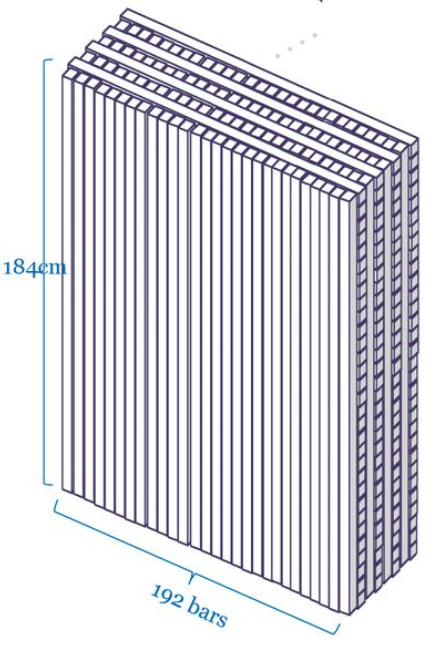
\includegraphics[width=0.3\linewidth]{FGD}
	\caption{The scheme of the exciting Fine-Grained Detector modules. Such a structure has a limited acceptance for the tracks at a high angle w.r.t. the beam.}
	\label{fig:up:sfgd:fgd}
\end{figure}

\section{Conceptual design}
A new target is going to be built with the optically isolated scintillator cubes. Each cube will have three holes in x, y, and z directions. The signal readout is organized with wavelength shifting fibers (WLS) that will transfer light to the Multi--Pixel Photo Counters (MPPC). With such a concept, the events will be reconstructed in three projections that can be further merged into a 3D image. The scheme of the concept is shown in \autoref{fig:up:sfgd:gen}.

\begin{figure}[!ht]
	\centering
	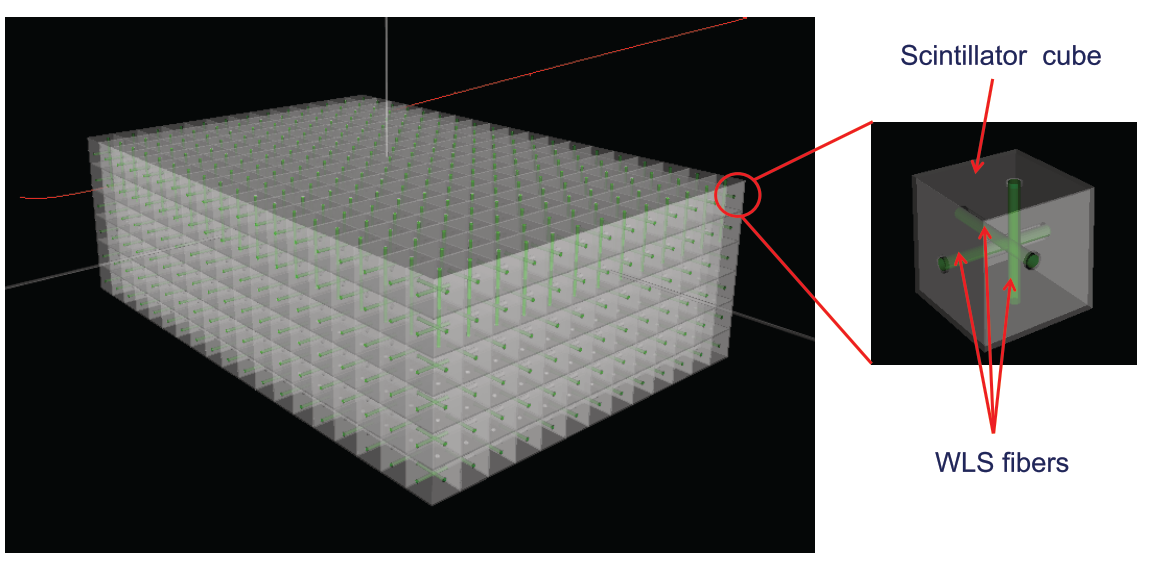
\includegraphics[width=0.8\linewidth]{sfgd_gen}
	\caption{The schematic concept of the SuperFGD detector made with scintillator cubes. Wavelength shifting fibers are used for the signal readout. The size of each cube is 1$\times$1$\times$1 $\text{cm}^3$.}
	\label{fig:up:sfgd:gen}
\end{figure}

High granularity is a strong advantage of the new detector. The measurements of the energy loss per length unit can estimate the type of self--contained particle with high accuracy. A low energy threshold for nucleon detection will gain the neutrino energy reconstruction accuracy and provide precise measurements of the neutrino interaction with matter.

The detector dimensions are \sfgdx{}$\times$\sfgdz{}$\times$\sfgdy{}  cubes 1$\times$1$\times$1 $\text{cm}^3$ each. The total number of cubes and channels will be 1 885 632 and 54 224 respectively. The fiducial mass of the ND280 will be nearly doubled with SuprrFGD. The details about the cube's characteristics are provided in \autoref{sec:up:sfgd:cube}. The MPPCs will be placed on the upstream, top, left and right side of the detector. The front--end electronics, including the digitizers, is going to be built on site. The digitized signal will be transported through the optical fiber outside the magnet to the ND280 data acquisition system. More details about the electronics can be found in \autoref{sec:up:sfgd:ele}.

\subsection{Scintillator cubes}
\label{sec:up:sfgd:cube}
The scintillator cubes are made from polystyrene doped with 1.5\% of paraterphenyl (PTP) and 0.01\% of POPOP. The cubes production is done with the injection molding with the press-form. Ten cubes could be produced at one act of molding that speeds up the mass production of the detector. The molding technology also increases the cube size accuracy comparing to the extrusion technology that is usually used for the scintillator detectors production. Cube dimensions accuracy is critical as we are going to assemble the detector from nearly 2 million cubes. Size fluctuations are required to be minimal to prevent cube's holes misalignment because of the position fluctuations.

\begin{figure}[!ht]
	\centering
	\begin{minipage}{0.40\linewidth}
		\centering
		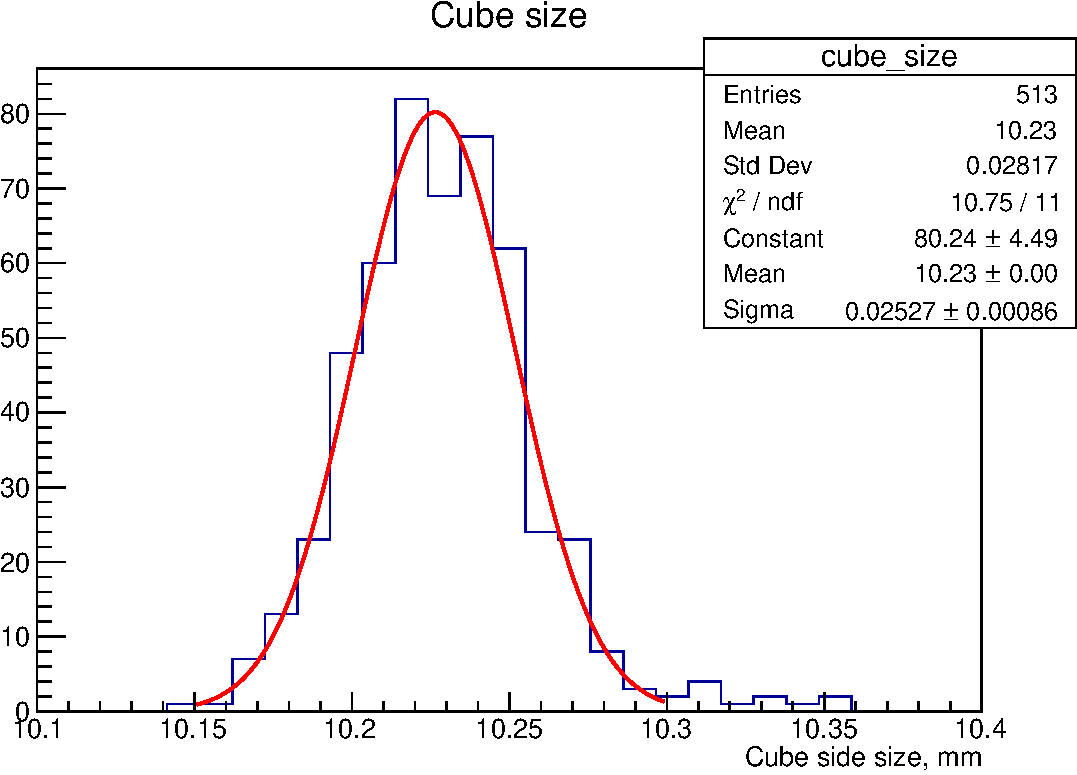
\includegraphics[width=\linewidth]{cube_size}
		\caption{The accuracy of the cube dimensions after the etching with a reflector. The results of 513 measurements are fit and demonstrates 25 $\mu$m accuracy.}
		\label{fig:up:sfgd:cube_s}
	\end{minipage}
	\begin{minipage}{0.19\linewidth}
	\hspace{\linewidth}
	\end{minipage}
	\begin{minipage}{0.40\linewidth}
		\centering
		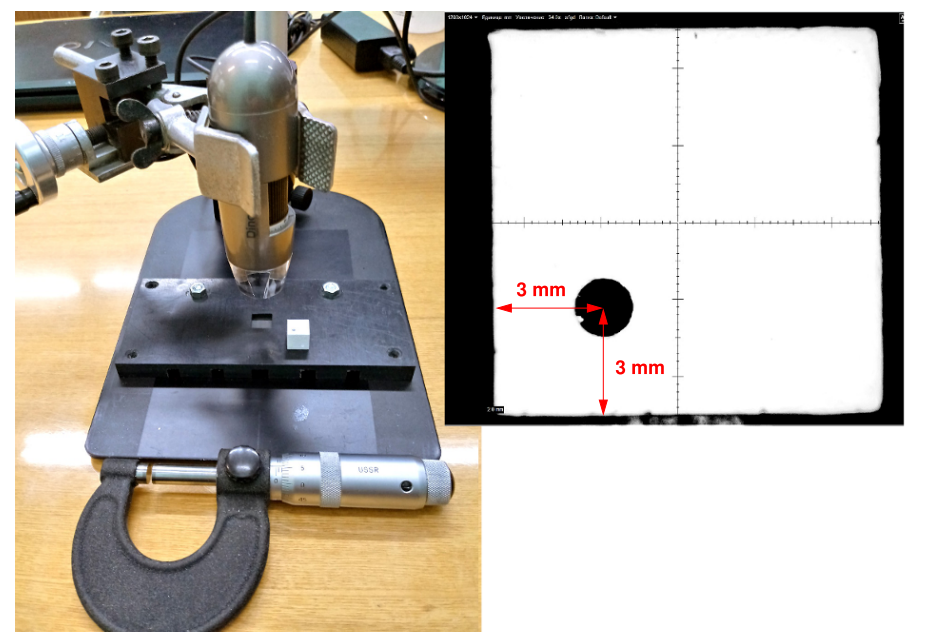
\includegraphics[width=\linewidth]{hole_measurements}
		\caption{The digital microscope used for the measurements of the hole position}
		\label{fig:up:sfgd:hole_pos}
	\end{minipage}
\end{figure}

After the molding, the cubes are covered by a chemical diffuse reflector by etching the scintillator surface in a chemical agent. The fluctuations of the cube size were measured after the etching procedure. The results are shown in \autoref{fig:up:sfgd:cube_s} and demonstrate the Gaussian behavior with 25 $\mu$m accuracy. Afterward, three holes with a 1.5 mm diameter are drilled. The positions of the holes are also precisely controlled with the digital microscope (\autoref{fig:up:sfgd:hole_pos}). Variations at the level of 80 $\mu$m were observed. Since the fiber diameter is 1 mm while the hole size is 1.5 mm, this is not supposed to bring a problem during the assembly. The cube size fluctuations remain the main challenge for the detector construction.

\subsection{Assembly}
\label{sec:up:sfgd:ass}
The assembly of the detector needs to be designed carefully. The setup requires aligning all the cubes at their position in three dimensions and easy insertion of the WLS fibers. With the given number of 2 million cubes and with measured uncertainties on cube size and hole positions, this is a challenging task.

\subsubsection{Loose structure}
We considered creating a loose structure of cubes self--aligned with fishing lines. The key idea is to fully assemble the detector with 1.2 mm fishing lines instead of the 1 mm WLS fibers. Cubes positions are fixed only with these lines without precise control over the position of each cube. Then the fishing line will be replaced one by one with the fibers. As WLS fiber diameter is smaller compared to the fishing line it should be easy to perform such a replacement. During the whole replacement, procedure cubes are aligned with lines and fibers. Such a technique will also protect the fibers that are quite expensive and fragile. They are going to be inserted only at the final stage of detector construction.

Detector assembly starts from the string construction (\autoref{fig:up:sfgd:string} (a)). A line of \sfgdx{} cubes is assembled on the fishing line. The set of \sfgdz{} strings is joint line by line to the plane \sfgdx{}$\times$\sfgdz{} (\autoref{fig:up:sfgd:string} (b)). Planes are put on top of each other to form a full detector (\autoref{fig:up:sfgd:string} (c)). The planes will be aligned so that the fishing lines will be inserted in the vertical holes as well. The alignment along the 3rd axis is the most difficult part of the assembly. The loose structure allows us to solve this problem with the small cube displacements during the insertion of the fishing line in the 3rd axis.

\begin{figure}[!ht]
	\centering
  \begin{minipage}{0.33\linewidth}
    \centering
    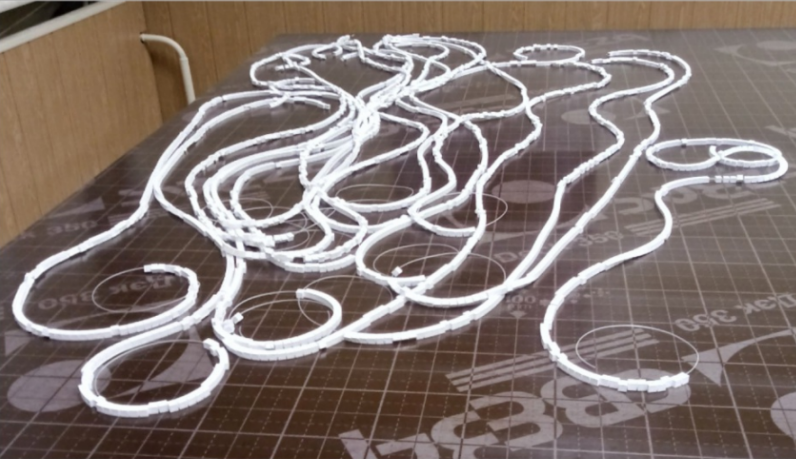
\includegraphics[width=\linewidth]{sfgd_FL_1} \\ (a)
  \end{minipage}
  \begin{minipage}{0.33\linewidth}
    \centering
    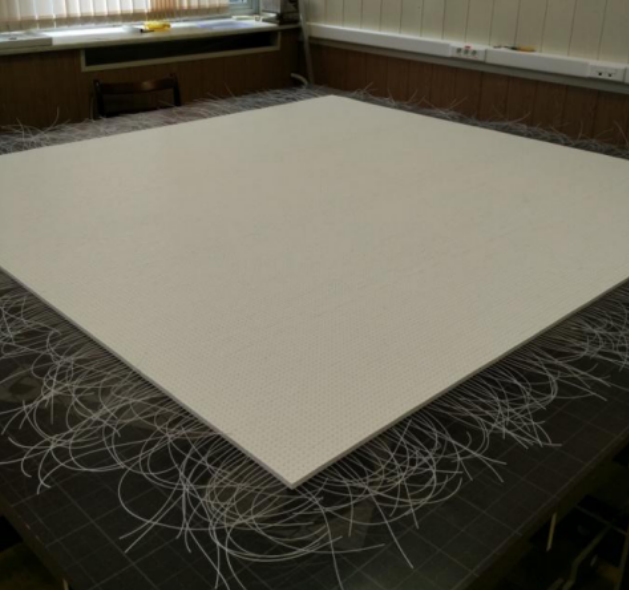
\includegraphics[width=\linewidth]{sfgd_FL_2} \\ (b)
  \end{minipage}
  \begin{minipage}{0.33\linewidth}
    \centering
    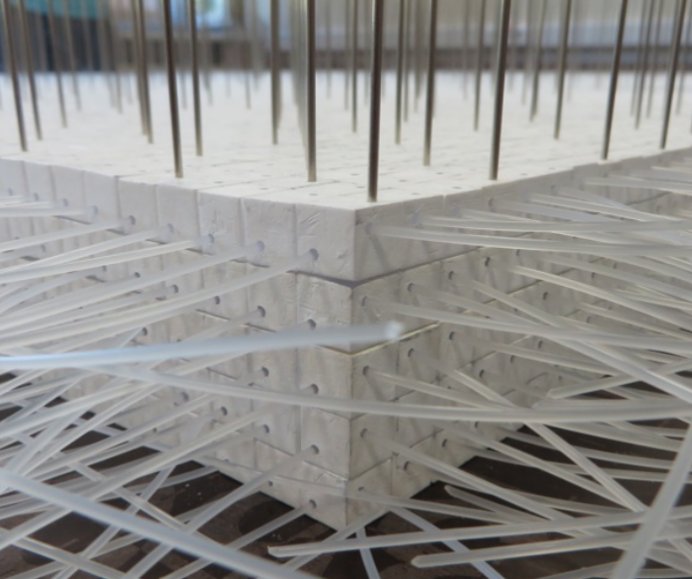
\includegraphics[width=\linewidth]{sfgd_FL_3} \\ (c)
  \end{minipage}
  \caption{The assembly technology of the SFGD detector with the fishing lines. The technology starts from the string assembly (a) that are further merged into the planes (b). Finally, the planes are put on top of the each other and the vertical holes are aligned with steel needles(c).}
  \label{fig:up:sfgd:string}
\end{figure}

Several tests of the assembly were performed. The first one includes a 2 m long prototype with the transversal dimensions 6$\times$6 cubes. This prototype was aimed to test the robustness of the assembly strategy, the possibility of the lines replacement with WLS, the length fluctuations of the 2 m long setup. The photos of the prototype are presented in \autoref{fig:up:sfgd:long}. With such a test it was proved that we can construct the detector with the proposed method. The tests were performed with and without a 50 kg payload on the top cover of the detector. In both cases, the fishing lines can be easily replaced by fibers. The friction of the fishing line with the 200 cubes is small and the line can be easily removed. There is no strong friction during fiber insertion as well. The length of the prototype was in agreement with the expectations within the 1 mm accuracy.

\begin{figure}[!ht]
	\centering
  \begin{minipage}{0.49\linewidth}
    \centering
    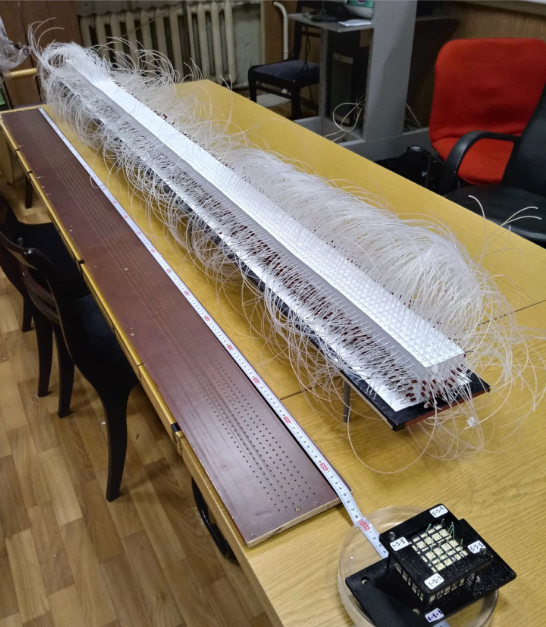
\includegraphics[width=0.5\linewidth]{sfgd_len_1} \\ (a)
  \end{minipage}
  \begin{minipage}{0.49\linewidth}
    \centering
    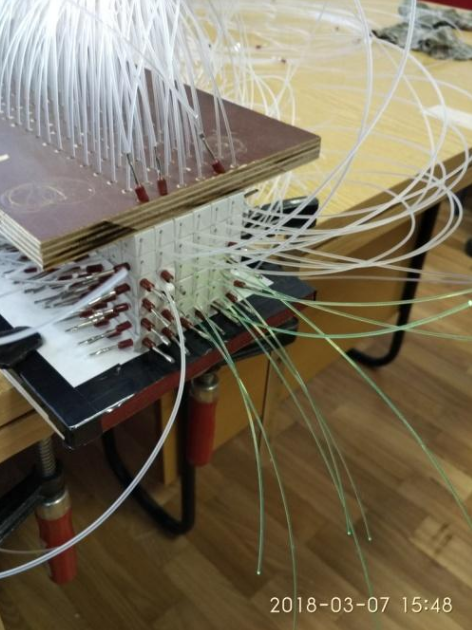
\includegraphics[width=0.5\linewidth]{sfgd_len_2} \\ (b)
  \end{minipage}
  \caption{Photos of the detector prototype built with 200$\times$6$\times$6 cubes. Cubes assembled with the fishing line (a) and after the replacement of several lines with WLS fibers (b).}
  \label{fig:up:sfgd:long}
\end{figure}

Two prototypes were built for the detector tests with the beam of charged particles. These prototypes served also as an assembly technology tests. The first one was quite small 5$\times$5$\times$5 cubes. The second one was slightly larger and contained 48$\times$24$\times$8 cubes. Details about prototypes construction and beamtest results will be overviewed in \autoref{sec:up:sfgd:beam}.

After the successful beamtests the tall ``tower'' was built with 15$\times$56$\times$192 cubes. The main purpose of this prototype was to test the possibility of the fishing lines replacement with the WLS fibers in a tall and long structure of cubes. It was confirmed that such a detector can be built with fishing lines and they can be replaced with the fibers afterward. The photo of the prototype is shown in \autoref{fig:up:sfgd:tall}. In addition, the test of the SuperFGD box strength and deformations was performed with this prototype. The details about the detector box will be provided in the next section.

\begin{figure}[!ht]
	\centering
	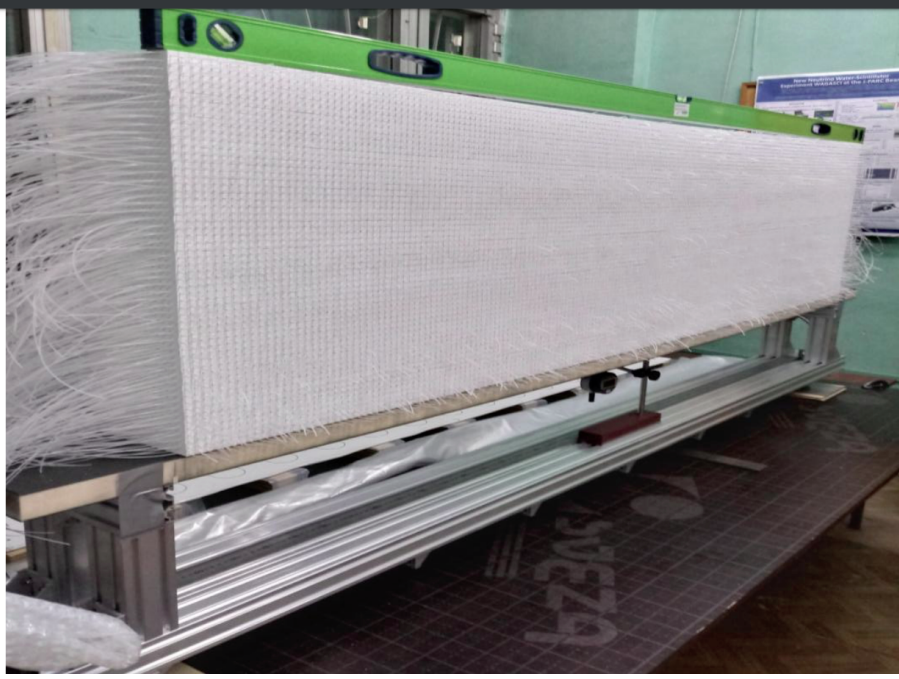
\includegraphics[width=0.3\linewidth]{sfgd_tall}
	\caption{The tall prototype of the SuperFGD detector made with 15$\times$56$\times$192 cubes.}
	\label{fig:up:sfgd:tall}
\end{figure}

\subsubsection{SuperFGD mechanics}
The mechanical structure of the scintillator target should provide a robust detector fixation to minimize the detector deformation due to load. The loose structure of cubes is a subject of deformation, while the WLS fibers are fragile and can be broken with the cube offset. At the same time, the dead space between the target and HA--TPC is desired to be as small as possible to gain the precision of charged particle tracking. The mechanical structure should provide the optical interface to readout all the channels and host the calibration system.

To meet these requirements, the walls of the box are made from 16 mm AIRAX core laminated with 2 mm CF skins and are screwed together. The box is drilled with 3 mm holes providing the exit for every WLS fiber. Three of the six walls carry the signal readout system. The MPPCs are soldered on printed circuit boards (PCB) that are screwed on the CF box. On the readout sides, the fibers are equipped with optical connectors to provide reliable light transfer to MPPC. The CAD of the optical interface and readout system is shown in \autoref{fig:up:sfgd:optics}. The other fibers endings are covered with the plastic coverage screwed to the box. This coverage shades the fibers from external light and also hosts the calibration system.

\begin{figure}[!ht]
	\centering
	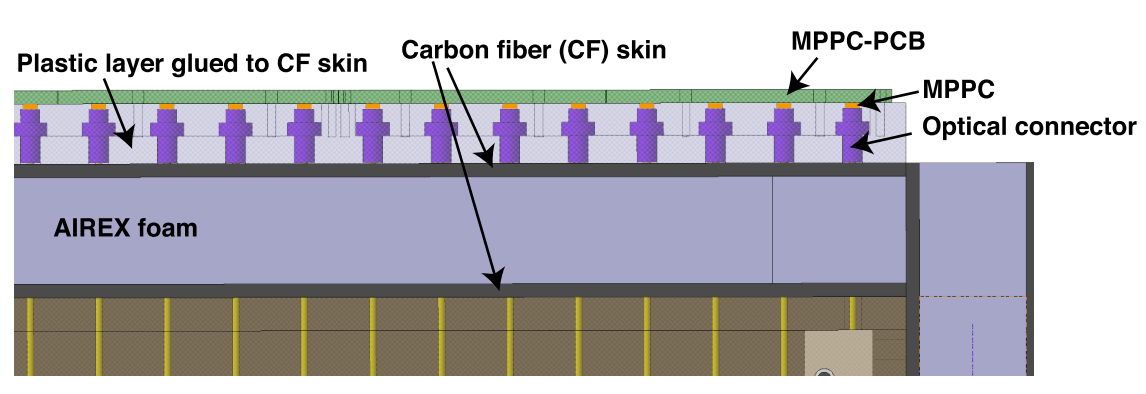
\includegraphics[width=0.7\linewidth]{optics}
	\caption{The optical interface of the SuperFGD detector}
	\label{fig:up:sfgd:optics}
\end{figure}

The deformation of the mechanical support structure was tested with the long and tall SuperFGD prototype (15$\times$56$\times$192 cubes). The measured sagitta was at the level of 20 mm. This value is close to the distance between the detectors but still meets the requirements and makes possible the detector assembly.

The calibration system is required to measure the MPPC gain, i.e. associate the output MPPC channel with the number of detected photoelectrons. In the current FGD, we use MPPC with a high noise rate that allows us to perform a calibration with the noise only. In the SuperFGD new low-noise MPPC will be used. It will make the signal cleaner, but will require the external light injection system for calibration. The Light Guide Plane (LGP) is used for this purpose. On the non-readout side of the fibers, the plastic plate is glued to the SuperFGD box. The light will be injected with LEDs at the plate border. The notches in the plate are made opposite to the fibers ends to scatter some light into the fibers (\autoref{fig:up:sfgd:calib}). With such a system the gain of each channel can be monitored continuously. It is especially important at the assembly stage to check all the MPPCs and fibers operate normally.

\begin{figure}[!ht]
	\centering
	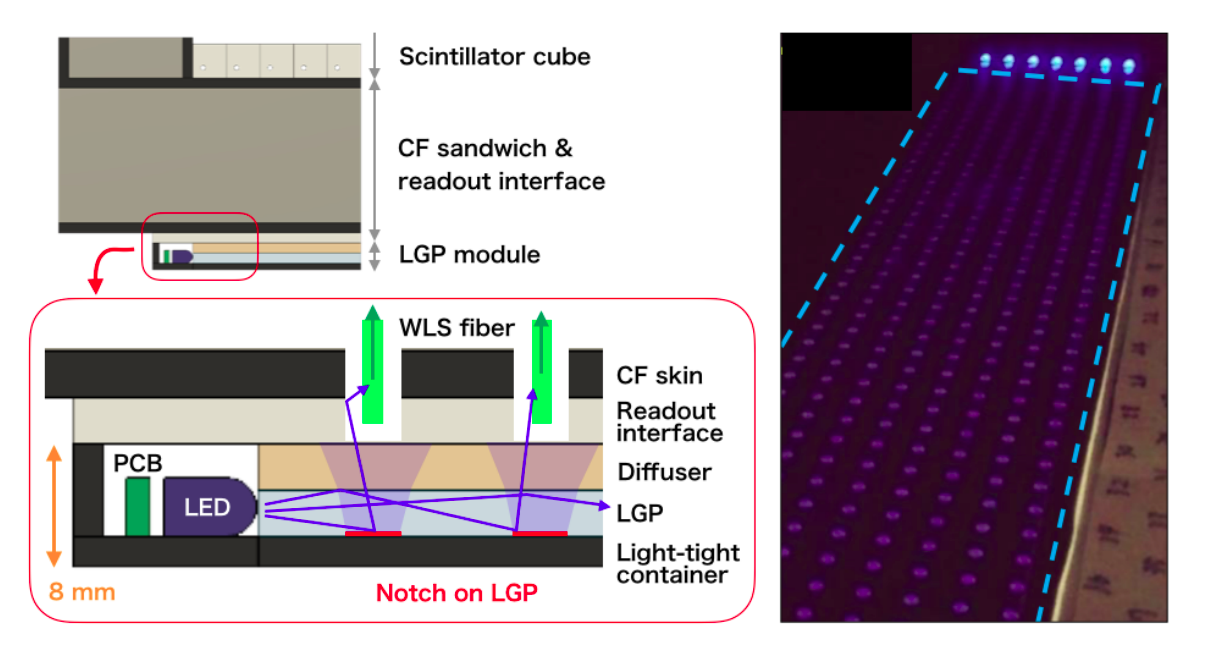
\includegraphics[width=0.7\linewidth]{calibration}
	\caption{SuperFGD calibration system with Light Guide Plane (left) and a LGP prototype (right).}
	\label{fig:up:sfgd:calib}
\end{figure}

\section{Electronics}
\label{sec:up:sfgd:ele}
SuperFGD electronics should measure the signal amplitude at every channel at every bunch of the neutrino beam. In T2K 8 bunches are separated with 600 ns and forms a spill that comes every 2 seconds. The readout system should be compatible with this regime. High dynamic range and precise timing are required for the precise physics measurement. Nucleons produced in the neutrino interactions are mostly low-energetic and stops shortly with large energy deposition. Since accurate energy measurements of the nucleons is required for the neutrino interactions measurements, a high dynamic range is essential. Time measurement is important for dividing particles directed to/from the target. The time-of-flight (ToF) system around the SFGD and HA--TPCs measures time with 100 ns accuracy. At our energies, the SFGD time resolution at the level of 1 ns is enough for the reliable estimation of the track direction.

The electronics system based on the CITIROC chips (Cherenkov Imaging Telescope Integrated Read Out Chip) was chosen as a baseline option. These chips are used in BabyMIND~\cite{Blondel2015b} experiment in the T2K near detector complex. Thus these chips were designed to operate with scintillator detector at the same neutrino beam and therefore are compatible with the beam timing. CITIROC electronics suits the requirements of the dynamic range and time resolution. It stores the signal in both low--gain and high--gain regime simultaneously and thus provides accurate amplitude measurements for both low and high light yield. At the moment, the bottle--neck of the dynamic range is a number of pixels in the MPPC. But our S13360-1325PE MPPCs carry 2668 pixels and this is more than enough for the precise measurements. The sampling rate of the CITIROC chip is 400 MHz (2.5 ns). That brings us below 1 ns time resolution per channel.

Front--End Boards (FEB) are mounted in towers on both sides of SGFD inside the magnet. PCBs are connected with the FEB with the coaxial cables. Such a scheme minimizes the dead material between the SFGD and HA--TPC. FEB provides signal amplification, digitization, and zero--suppression. The optical cable transmits the data outside the magnet to the ND280 global DAQ system. This connection serves for the time synchronization as well.

\section{Simulations}
\label{sec:up:sfgd_sim}
To estimate the behavior and main physical characteristics of the future detector we performed a bunch of simulations. The framework based on Geant4~\cite{Agostinelli2003} toolkit was created to perform a Monte--Carlo simulation of the proposed detector~\cite{ndUpRepo}. The detector response was estimated based on the well-known behavior of the scintillator detector FGD. Further corrections based on the test beam data are considered. The geometry of the cubes with holes, instrumented with WLS fibers was fully implemented in the framework. The visualization of the simulated geometry is shown in \autoref{fig:up:sfgd:gen}. The propagation and interactions of the particles in the detector are carried out by Geant4 toolkit. As an output, we know the energy spent on the ionization in the scintillator material.

Based on the known energy loss in the scintillator we estimated the amount of light measured by the MPPC. The first step is evaluating the amount of ionization energy that went to light emission. The empirical Birks law was used for this purpose~\cite{Birks1951}.

\begin{equation}
\frac{dS}{dr}=\frac{dE/dr}{1+k_B\times dE/dr}
\end{equation}
where $k_B=0.0208\text{cm/MeV}$ is a Birks constant that was precisely measured for the plastic scintillators. Based on the total energy spent on light emission we estimate the number of photons produced and captured with the WLS fibers. Based on our experience with FGD we started with the value of 156.42 $\gamma$/MeV. This value is supposed to be tuned later with the beamtest data. The attenuation of the light in the fiber is estimated with the exponential law (\autoref{eq:att}).

\begin{equation}
\label{eq:att}
L\times=a\cdot e^{-x/L_{long}}+(1-a)\cdot e^{-x/L_{short}}
\end{equation}
where $L_{long}$ and $L_{short}$ are 2 attenuation length and $a$ is their relative strength. As before, we have some knowledge about the attenuation length from the FGD operation. In addition, the measurements of the attenuation length in our fiber type were performed with LED. Attenuation parameters were set to $a=0.77$, $L_{long}=4634$ mm, $L_{short}=332$ mm. The MMPC photodetection efficiency is specified by its manufacturer at 25\%. Thus the energy deposited by a charged particle is transformed into the number of detected photo electrons. A similar approach is used in the simulation of the FGD in the ND280.

\subsection{Expected light yield and PID}
\subsubsection{Simulation cross--check}
One of the goals of the simulations is to estimate the light yield of the detector with different particle types. We want to be sure that the dynamic range of the MPPC is suitable for the amount of light that is going to be measured. First of all, we compared the results of the simulation with the results of the first beam test (\autoref{sec:up:sfgd:beam1}). I found that with our simulation we expect to observe 41 photo electrons per channel in the first small SuperFGD prototype with the beam at the CERN T10 area (mostly Minimum Ionizing particles (MIP)). In the data, we observed a very similar result --- 42 p.e. per channel. Thus we decided that the simulation parameters are reliable enough.

\subsubsection{Beamtest simulations}
After the validation of the simulation parameters with the first beamtest we simulate the signal from the second prototype (\autoref{sec:up:sfgd:beam2}). The main goal is to estimate the detector response for through-going MIP particles and stopping protons. As we expect a large energy deposition in the second case, our detector should be able to measure high signal amplitude. Simulated event displays are shown in \autoref{fig:up:sfgd:sim_scnd}.

\begin{figure}[!ht]
	\centering
	\begin{minipage}{0.33\linewidth}
		\centering
		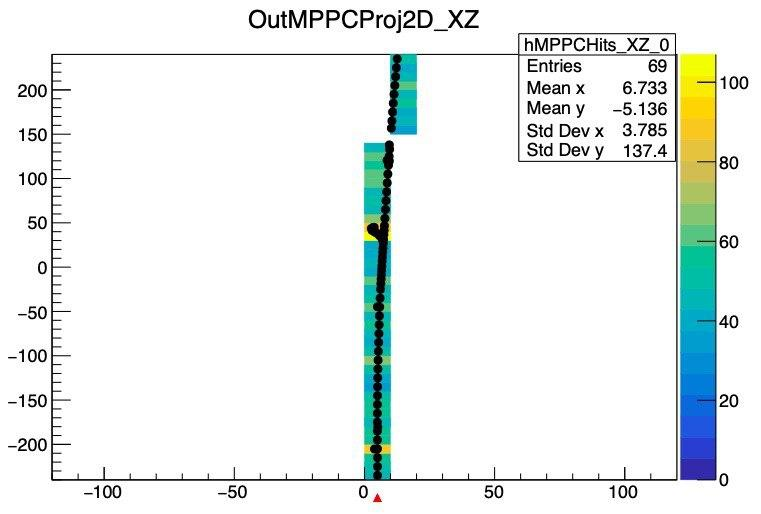
\includegraphics[width=\linewidth]{scnd_pion_sim} \\ (a)
	\end{minipage}
	\begin{minipage}{0.33\linewidth}
		\centering
		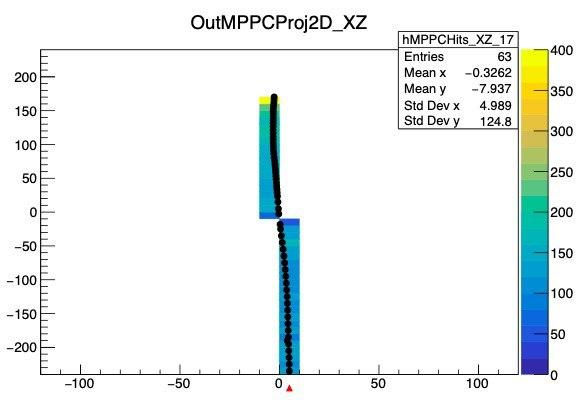
\includegraphics[width=\linewidth]{scnd_proton_sim} \\ (b)
	\end{minipage}
	\begin{minipage}{0.33\linewidth}
		\centering
		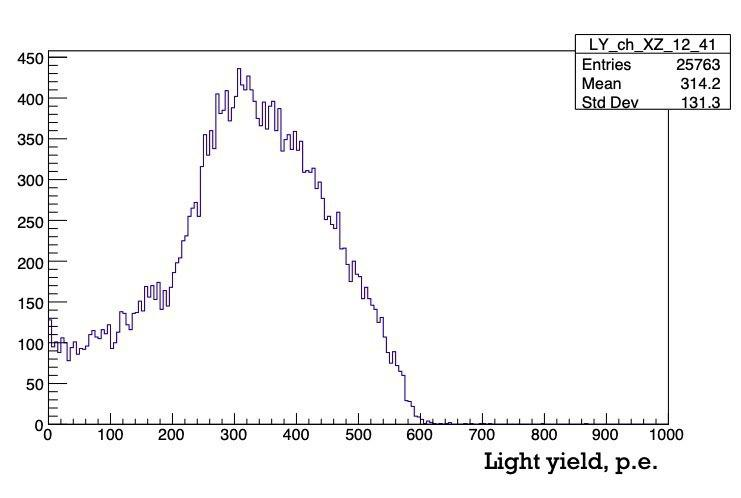
\includegraphics[width=\linewidth]{scnd_pr_last} \\ (c)
	\end{minipage}
	\caption{The simulations of the second prototype of the SFGD detector. Event displays of the through-going 1 GeV/c pion track (a) and a stopping proton track (b). The light yield distribution in the stopping proton last cube (c).}
	\label{fig:up:sfgd:sim_scnd}
\end{figure}

I estimated the light yield from the through-going MIP track at a value of 50 p.e.. The value is similar to the measurements done with the first prototype and is sufficient for the tracking and time resolution measurements. The signal from the stopping proton is much higher and reaches 600 p.e.. The majority of the prototype's channels are equipped with MPPC with a dynamic range of 2668 pixels that is more than enough for successful energy measurements.

\subsubsection{PID studies}
As mentioned before, with SuperFGD we can determine the type of self-contained particle by the energy loss. We performed a simulation to study the accuracy of such a determination. The effect of light attenuation should also be studied. As we are using 2 m long fibers, the attenuation may be quite severe and affect particle identification. I performed simulations of the propagation of different particles through the detector. The samples with the different initial locations of the particles were considered: close to the MPPC, excluding the attenuation effect and at the far corner of the detector where the attenuation is the strongest. The ionization energy loss estimated for muon and proton in both positions is shown in \autoref{fig:up:sfgd:pid}. The particle momenta are taken from the neutrino interactions simulated with GENIE generator. The cut was put at the value where muon and proton PDF intersects. Thus the efficiency and purity of the muon selection can be estimated. As one can see the quality of the selection depends very weak from the initial particle position. The light attenuation reduces the total amount of light but doesn't spoil the particle identification. These plots also demonstrate a good PID power of the detector even with a simple comparison of dE/dx. More sophisticated selection using a momentum by range can further improve the accuracy of particles separation.

\begin{figure}[!ht]
	\centering
	\begin{minipage}{0.25\linewidth}
		\centering
		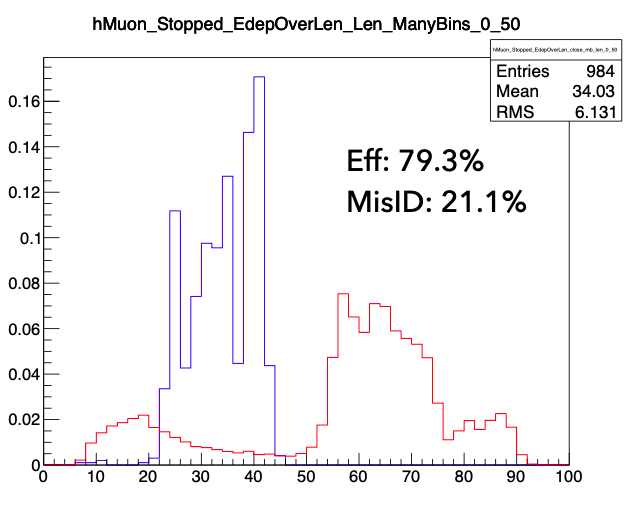
\includegraphics[width=\linewidth]{PID_1}
	\end{minipage}
	\begin{minipage}{0.25\linewidth}
		\centering
		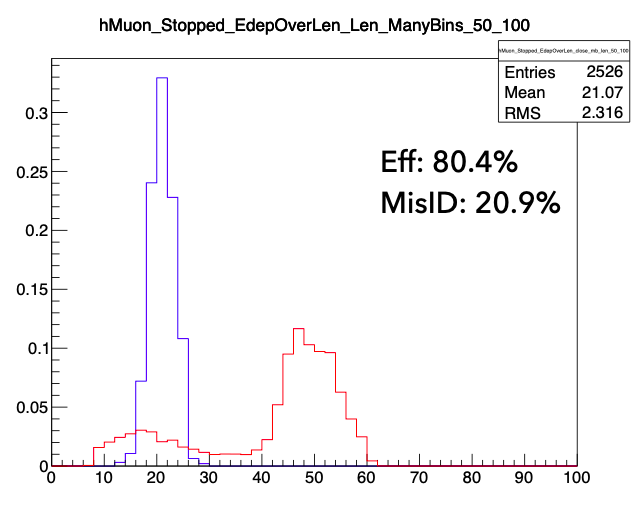
\includegraphics[width=\linewidth]{PID_2}
	\end{minipage}
	\begin{minipage}{0.25\linewidth}
		\centering
		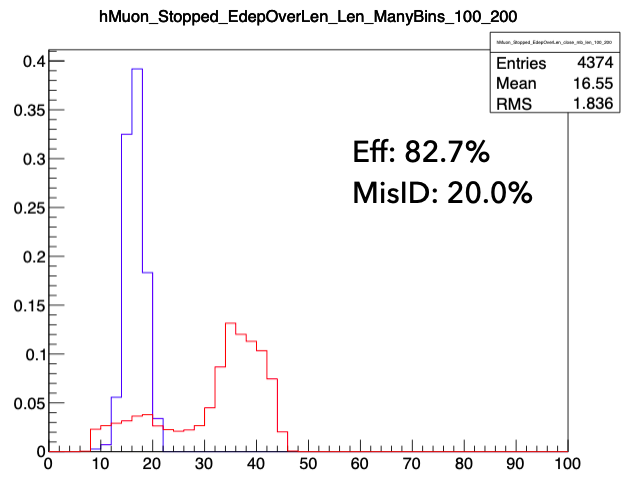
\includegraphics[width=\linewidth]{PID_3}
	\end{minipage}
	\hfill
	\begin{minipage}{0.25\linewidth}
		\centering
		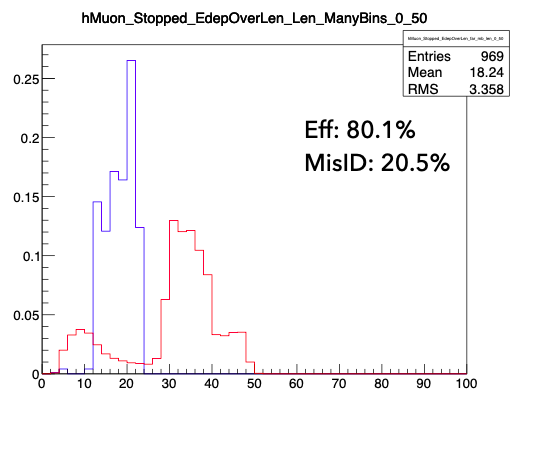
\includegraphics[width=\linewidth]{PID_4} \\ $ L < 50$ mm
	\end{minipage}
	\begin{minipage}{0.25\linewidth}
		\centering
		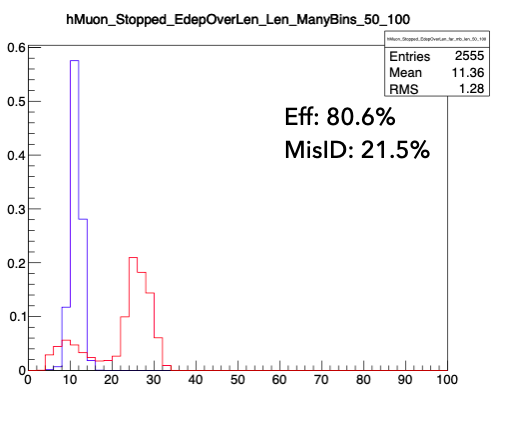
\includegraphics[width=\linewidth]{PID_5} \\ $50 < L < 100$ mm
	\end{minipage}
	\begin{minipage}{0.25\linewidth}
		\centering
		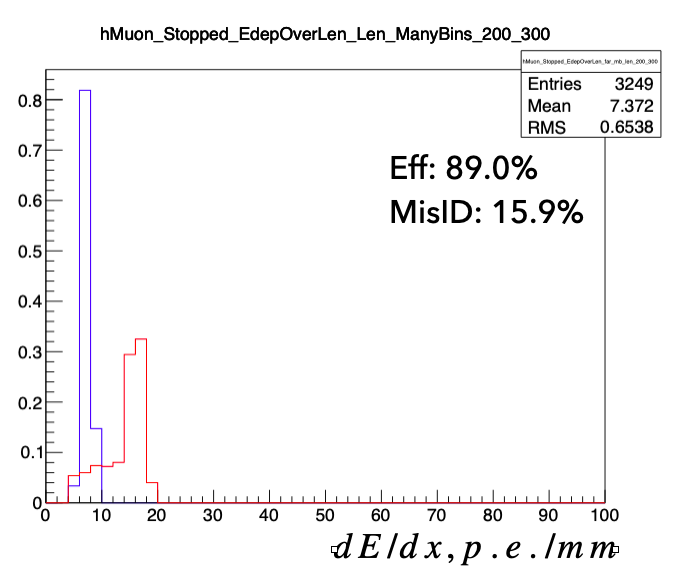
\includegraphics[width=\linewidth]{PID_6} \\  $100 < L < 200$ mm
	\end{minipage}
	\caption{The energy loss per length unit PDFs for muon (blue) and proton(red) for different track length and at different distances from MPPCs. Top row corresponds to the particle position close to MPPC and bottom row corresponds to position far away from MPPC so the light attenuation in fiber is the strongest. The efficiencies of the muon identification as well as a rate of the misidentified protons is shown.}
	\label{fig:up:sfgd:pid}
\end{figure}

\subsection{Pileups}
\label{sec:up:sfgd:pu}
Neutrino interactions happen not only in the fiducial material but also in the concrete of the pit, in the magnet coil of the ND280 and in the other detectors. SuperFGD will suffer from the pile ups as the particles from such interactions could enter the detector and overlap with the signal from the neutrino interactions inside the fiducial volume. I estimated the rate of pile ups for different beam intensities. Simulation of the neutrino interactions outside of the basket was already done and widely used in the experiment. I used this sample and cherry picked tracks that entered the basket and are pointed towards SuperFGD. Such tracks are used as an input for the SuperFGD simulation framework to estimate detector response. The results are overlapped with the simulation of the neutrino interactions inside SuperFGD. Finally, we got the fraction of pileuped events in the whole detector and a fraction of pileuped channels in 2D projections. The results are summarized in \autoref{tbl:up:sfgd:pile_up}. Two beam powers are considered 500 and 1000 kW.

\begin{table}[!ht]
	\begin{tabular}{|l|ccccc|}
	\multicolumn{6}{l}{For $10^{21}$ POT total number of $\nu$ events in neutrino mode in  SFGD: 234 546} \\
	\hline
	Beam  					& \multicolumn{5}{c}{Pile ups in:} \\
	power, kW				& whole detector 	& certain cube 	& XY projection 	& YZ projection 	& XZ projection \\
	\hline
	500							& 11 520					& 0.64  				& 14.09					  & 9.95 						& 55.58 \\
	1000 						& 22 147 					& 1.28 					& 28.12 					& 19.91 					& 111.17 \\
	\hline
	\hline
	\multicolumn{6}{l}{} \\
	\multicolumn{6}{l}{For $10^{21}$ POT total number of $\overline{\nu}$ events in anti-neutrino mode in SFGD: 60 837} \\
	\hline
	Beam  					& \multicolumn{5}{c}{Pile ups in:} \\
	power, kW				& whole detector 	& certain cube 	& XY projection 	& YZ projection 	& XZ projection \\
	\hline
	500							&  1 382					& 1.01  				&  2.43					  & 2.17  					& 10.90 \\
	1000 						&  2 659 					& 1.93 					&  4.68 					& 4.17   					& 21.00 \\
	\hline
	\end{tabular}
	\caption{The pile up rate in the SuperFGD detector.}
	\label{tbl:up:sfgd:pile_up}
\end{table}

The YZ plane has a lower pile up rate as it has the largest number of channels and coincidence is less probable. XY plane contains the least number of channels, but the pile up rate is lower comparing to XZ plane. Most of the OOFV particles are going downstream that's why their tracks are extended along the Z axis and the coincidence of channel in XZ projection is more probable. In total, the rate of the channels pile up with the out of fiducial volume tracks is low and will not affect the data quality.

\section{Beamtest}
\label{sec:up:sfgd:beam}
Several beamtests were performed to evaluate the detector performance and characteristics.

\subsection{First CERN beamtest}
\label{sec:up:sfgd:beam1}
The first ever test was done with the small 5$\times$5$\times$5 cubes prototype. The main goals of the test were the first measurement of the light yield and time resolution with the beam of charged particles. A photo of the first prototype is shown in \autoref{fig:up:sfgd:1st}.

\begin{figure}[!ht]
	\centering
	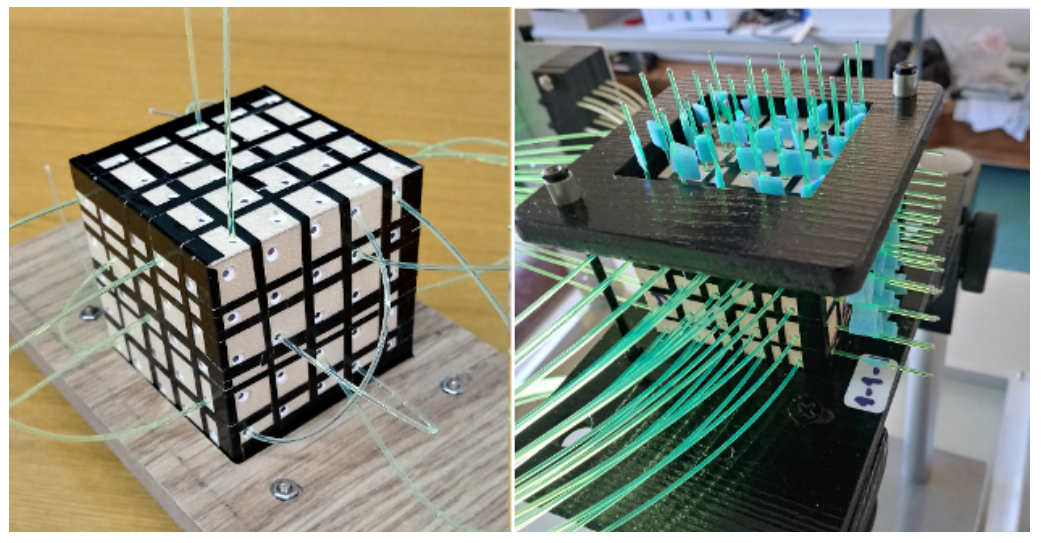
\includegraphics[width=0.5\linewidth]{fst_photo}
	\caption{The first 5$\times$5$\times$5 cubes prototype of the SuperFGS detector. The assembly stage (left) and a complete prototype with inserted WLS readout fibers (right).}
	\label{fig:up:sfgd:1st}
\end{figure}

The beamtest was performed at the T10 area of the CERN Proton Synchrotron (PS). The 6 GeV/c beam consisted mostly of positron and protons. Two scintillator bars were installed in 26 cm before and after the prototype and used as a trigger and reference measurements for the time resolution studies.

The light was readout with two fibers perpendicular to the beam direction, fibers along the beam were not inserted. The distribution of the sum of the light yield from both channels is shown in \autoref{fig:up:sfgd:1st_res} (a). So we observed in average 80 photo electrons from one cube that is enough for the particle tracking and accurate time measurements. The time resolution was measured with respect to both trigger bars. A 5 GHz digitizer was used for sampling the data from the detector. Combing the measurements from two fibers in the same cube we reached a time resolution at the level of 650 ps (\autoref{fig:up:sfgd:1st_res} b) and the resolution of the single channel is 0.95 ns. This result is beyond the minimal requirements and opens a way towards precise ToF measurements inside the SFGD that may be used for the neutron energy measurements (see \autoref{ch:up:neutron}).

\begin{figure}[!ht]
	\centering
	\begin{minipage}{0.49\linewidth}
		\centering
		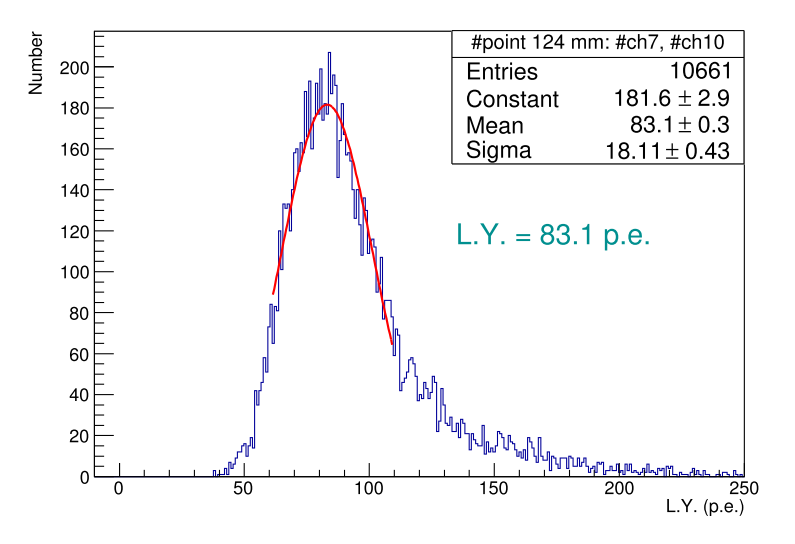
\includegraphics[width=\linewidth]{fst_light} \\ (a)
	\end{minipage}
	\begin{minipage}{0.49\linewidth}
		\centering
		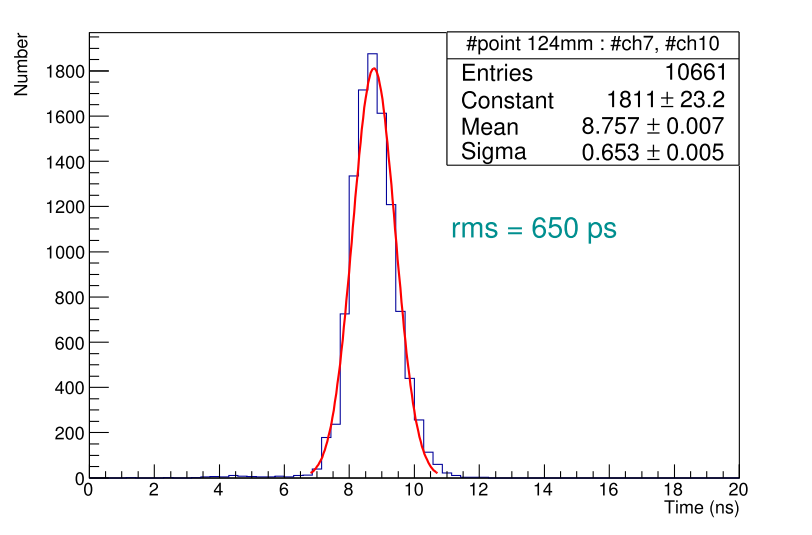
\includegraphics[width=\linewidth]{fst_time} \\ (b)
	\end{minipage}
	\caption{A light yield (a) and a time resolution (b) of the first prototype of the SuperFGD detector.}
	\label{fig:up:sfgd:1st_res}
\end{figure}

The results of the beam test were published in~\cite{Mineev2019}.

\subsection{Second CERN beamtest}
\label{sec:up:sfgd:beam2}
The first small prototype was used to test the concept and measure basic detector characteristic. More sophisticated tests are required to study setup performance with different particle types at various energies. The second prototype was made of 48$\times$24$\times$8 cubes. The size a driven by the size of the magnet in which it would be placed. In this larger version all the channels were instrumented with fibers and MPPCs. The readout was organized with CITIROC electronics that is going to be used in the full scale detector. The photos of the setup are shown in \autoref{fig:up:sfgd:scnd_photo}.

\begin{figure}[!ht]
	\centering
	\begin{minipage}{0.26\linewidth}
		\centering
		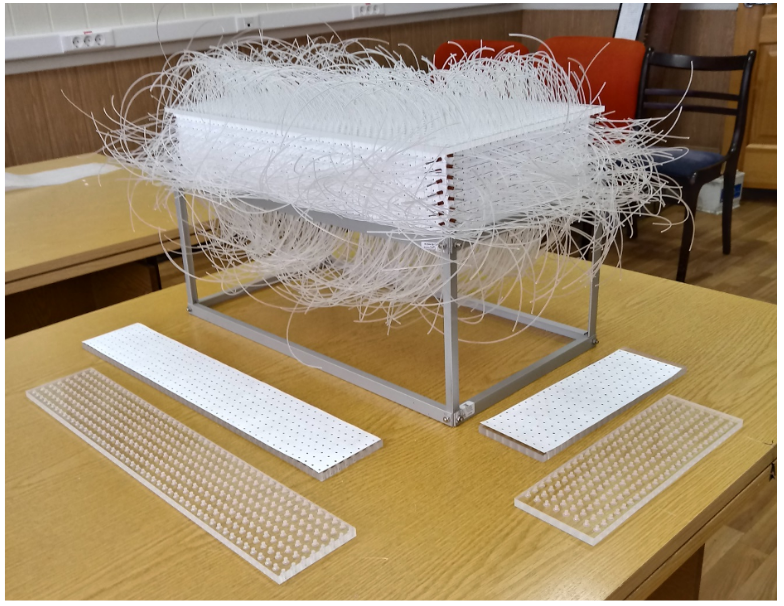
\includegraphics[width=\linewidth]{scnd_ass} \\ (a)
	\end{minipage}
	\begin{minipage}{0.36\linewidth}
		\centering
		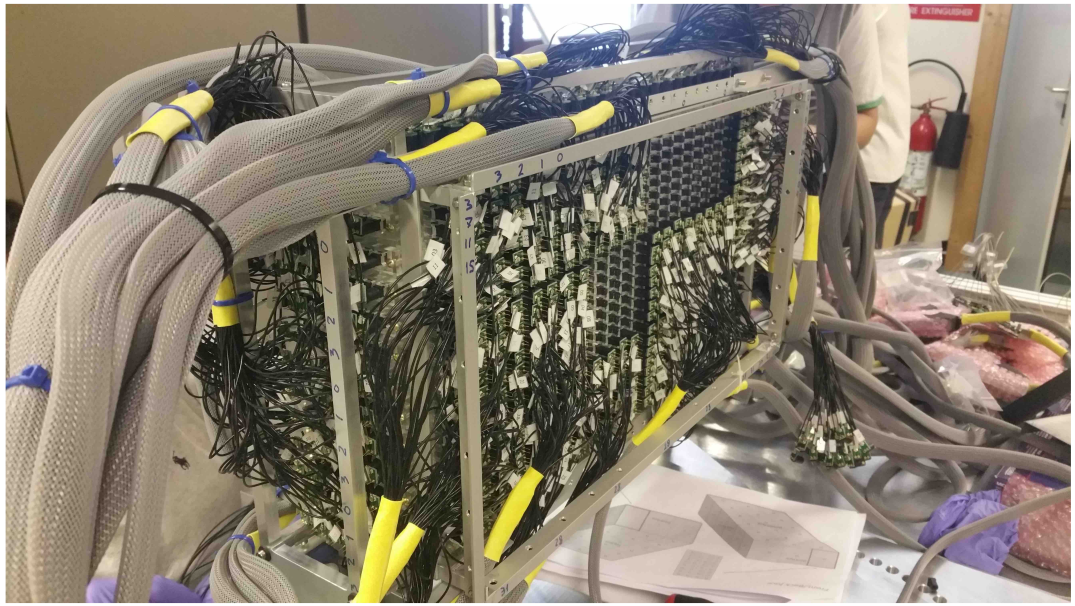
\includegraphics[width=\linewidth]{scnd_inst} \\ (b)
	\end{minipage}
	\begin{minipage}{0.36\linewidth}
		\centering
		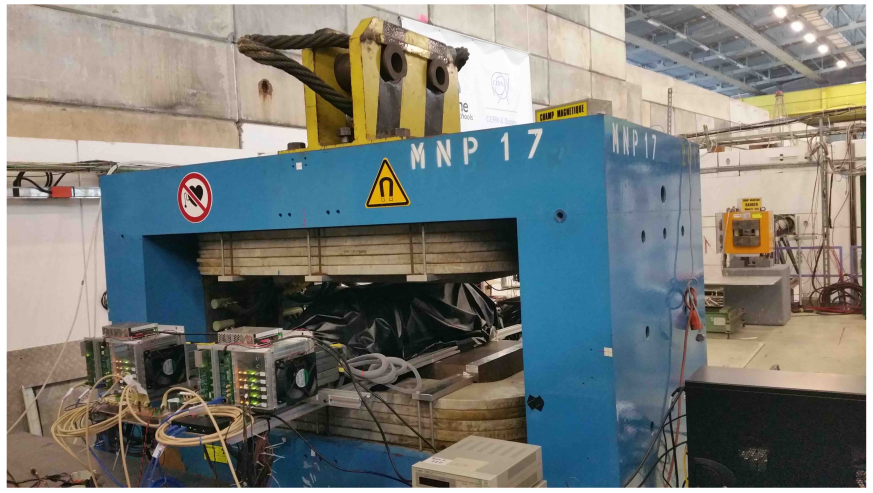
\includegraphics[width=\linewidth]{scnd_magnet} \\ (c)
	\end{minipage}
	\caption{The second SuperFGD prototype made of 48$\times$24$\times$8 cubes. During the assembly with fishing lines (a), fully instrumented with WLS fibers, MPPCs and cabled (b), installed in the magnet at the beamline (c).}
	\label{fig:up:sfgd:scnd_photo}
\end{figure}

The test was performed at the T9 area at Proton Synchrotron (PS) beamline at CERN. The beam parameters are similar to what was described in the TPC beamtest chapter (\autoref{sec:up:tpc:cern} of \autoref{ch:up:tpc}). The beam is composed of electrons, pions, and protons with a momentum that varies from 800 MeV/c up to 6 GeV/c. Thus we can observe a through going MIP tracks as well as more complicated topologies like single photon production and conversion, electromagnetic shower, stopping proton. All these events are likely to happen in the ND280 detector and it is interesting to study them with the prototype. Some event displays are shown in \autoref{fig:up:sfgd:scnd_ed}.

\begin{figure}[!ht]
	\centering
	\begin{minipage}{0.49\linewidth}
		\centering
		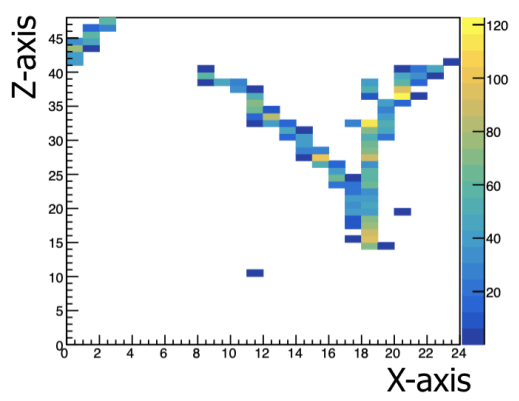
\includegraphics[width=\linewidth]{ed_photon} \\ (a)
	\end{minipage}
	\begin{minipage}{0.49\linewidth}
		\centering
		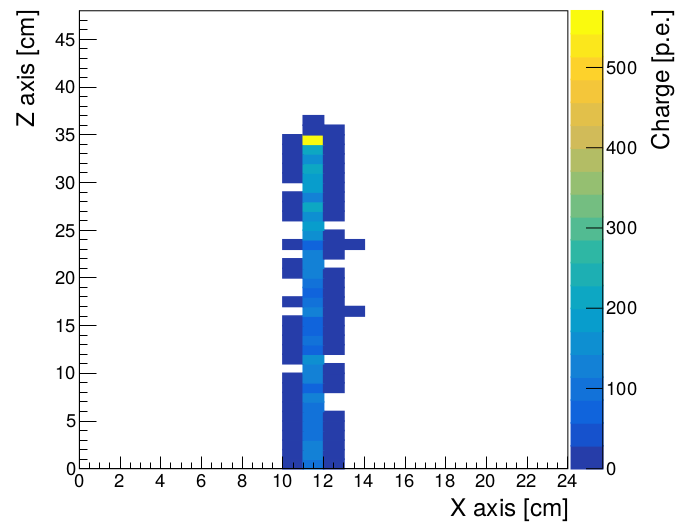
\includegraphics[width=\linewidth]{ed_proton} \\ (b)
	\end{minipage}
	\caption{Event displays from the second prototype of the SUperFGD detector. A photon production and conversion into electron--positron pair (a) and a stopping proton track (b)}
	\label{fig:up:sfgd:scnd_ed}
\end{figure}

The analysis started with estimating the basic detector characteristics like the light yield (LY) and time resolution. The LY was studied with the 0.8 GeV/c MIP sample. The light attenuation in the fibers is not negligible in our detector. Hence we first measured the attenuation effect and then apply the correction to each measurement based on the distance between an illuminated cube and a MPPC. Therefore the obtained value that characterizes a light production and collection in the cube and does not depend on cube position inside the detector. The attenuation was measured for fibers perpendicular to the beam directions. The observed light follows the exponential law with respect to the distance from the cube to the MPPC. The parameters of the exponential law are extracted from the fit and further used for correction of the measured light. The attenuation with respect to the travel distance of the light in the fiber is shown in \autoref{fig:up:sfgd:scnd_light} (a). The corrected values of the LY per cube are shown in \autoref{fig:up:sfgd:scnd_light}.

\begin{figure}[!ht]
	\centering
	\begin{minipage}{0.49\linewidth}
		\centering
		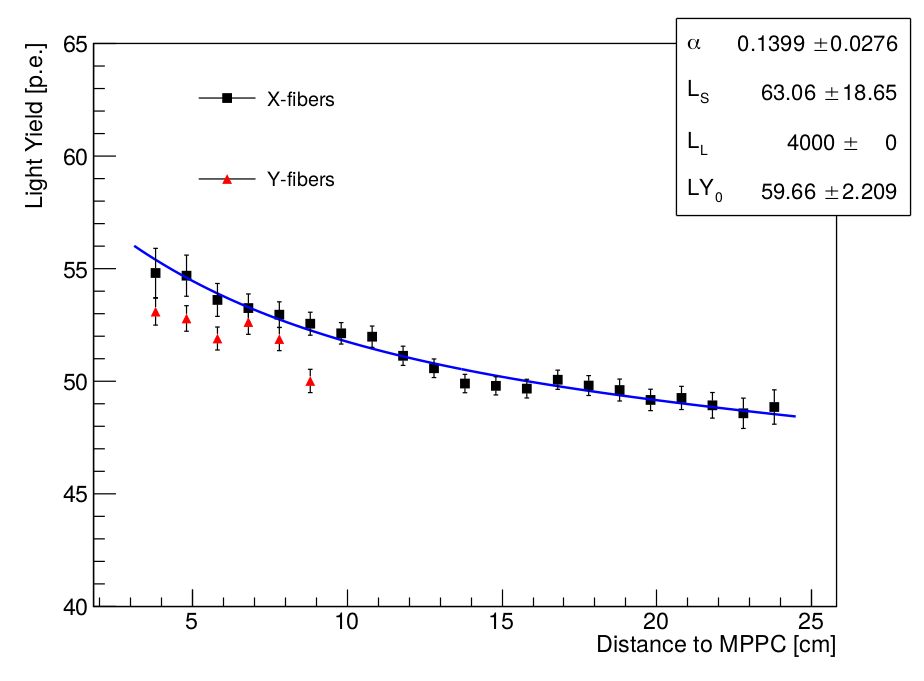
\includegraphics[width=\linewidth]{scnd_att} \\ (a)
	\end{minipage}
	\begin{minipage}{0.49\linewidth}
		\centering
		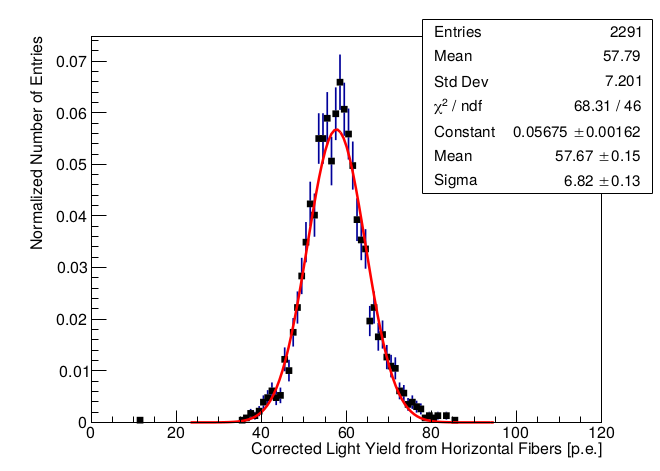
\includegraphics[width=\linewidth]{scnd_ly} \\ (b)
	\end{minipage}
	\caption{The attenuation of the light in the fibers (a) is used to estimate the light yield of the cube (b).}
	\label{fig:up:sfgd:scnd_light}
\end{figure}

The measurements of the time resolution were done separately for short and long fibers (8 and 24 cm respectively). The trigger that was used during the test was not precise. It has an uncertainty much more than 1 ns, thus can not be used as a reference. Instead, the measurements in the particular cube were compared to the cube in the middle of the prototype (in the 24 layer of 48). The uncertainty is supposed the same for both and the final time resolution is $\sqrt{2}$ times smaller than the smearing of the $\Delta T=T_{cube}-T_{reference}$. The distribution of the time resolution across different channels and different fiber length is shown in \autoref{fig:up:sfgd:scnd_time}. The obtained result is a bit worse than 1 ns. Some channels tend to have worse resolution forming a distribution with a long tail. This result is slightly worse compared to the resolution obtained with the first prototype (0.95 ns). In the second test, the CITIROC electronics with 400 MHz sampling was used, while in the first test we used 5 GHz digitizer and that may be the main reason for the different results.

\begin{figure}[!ht]
	\centering
	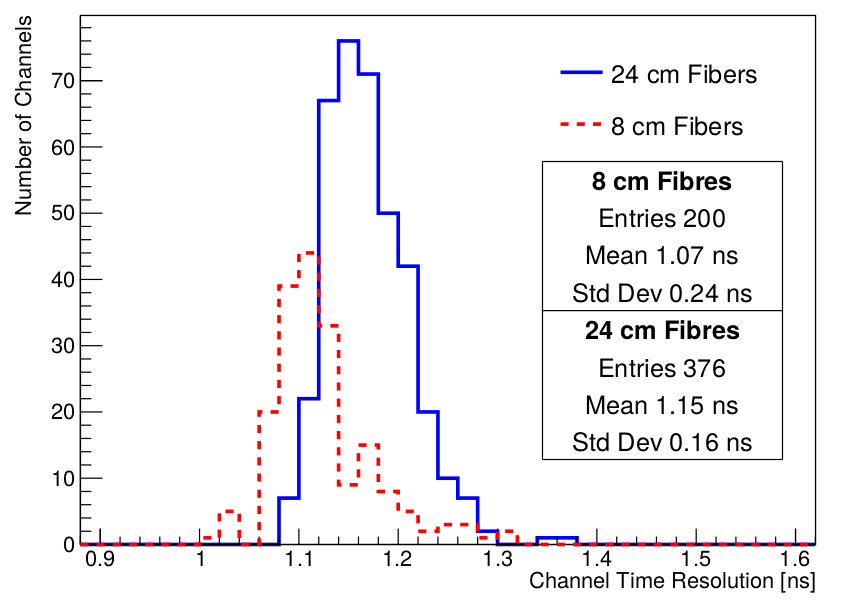
\includegraphics[width=0.4\linewidth]{scnd_time}
	\caption{The time resolution of the second prototype of the SuperFGD detector measured independently for every channel and fiber length.}
	\label{fig:up:sfgd:scnd_time}
\end{figure}

A bunch of physics measurements was performed with the prototype. As we have a composition of different particles, we can plot the energy loss per length unit (dE/dx) and to study how well samples are separated. It will demonstrate the possibility of the detector to distinguish types of self-contained particles. Before the external detector like a TPC was required. The information from the trigger was used to distinguish muon/pion, electron, and proton samples. The energy losses per each sample are shown in \autoref{fig:up:sfgd:scnd_dedx}.

\begin{figure}[!ht]
	\centering
	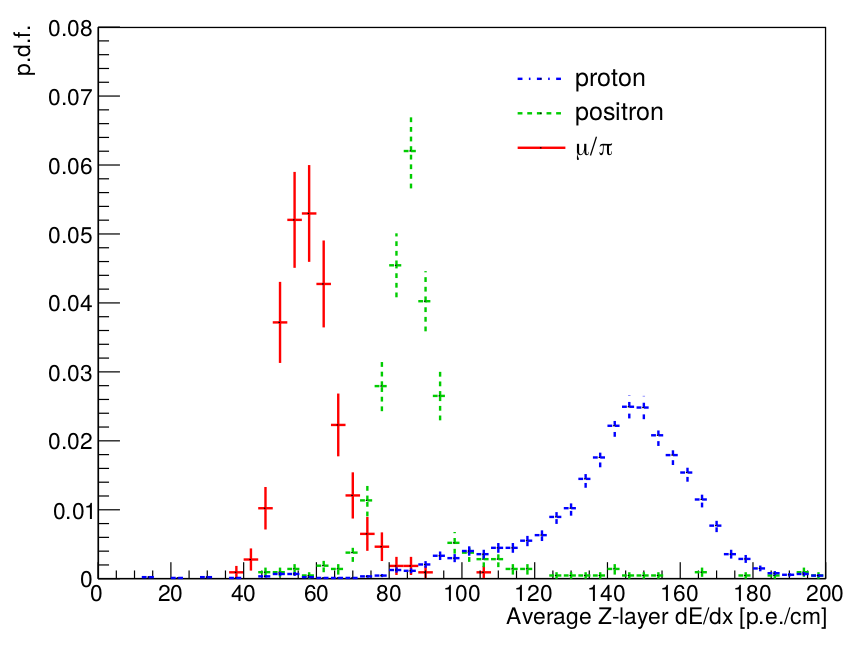
\includegraphics[width=0.4\linewidth]{scnd_dedx}
	\caption{The energy loss per length unit (dE/dx) for different particles samples distinguished by the trigger type. 0.8 GeV/c muon/pion and proton samples and 1 GeV/c positron sample were used.}
	\label{fig:up:sfgd:scnd_dedx}
\end{figure}

The other interesting sample is stopping protons. The energy deposition rises at the end of the proton track (Bragg peak) and results in a large light deposition. Since we are going to measure low energy protons from neutrino interactions it is interesting to see the detector response for such a sample. We used a 0.8 GeV/c protons as the minimal momentum that could be selected with the beamline. The energy deposition of the proton, positron , and muon/pion along their track is shown in \autoref{fig:up:sfgd:scnd_pr}. On this plot, the Bragg peak is clearly seen. The dynamic range of MPPCs used in the test is enough to measure light deposition.

\begin{figure}[!ht]
	\centering
	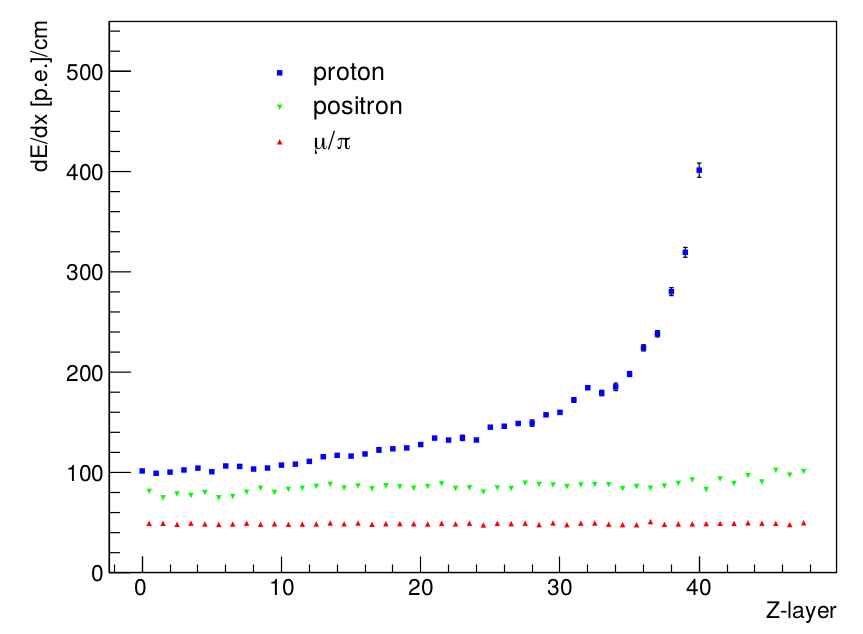
\includegraphics[width=0.4\linewidth]{scnd_pr}
	\caption{The energy deposition along the track for different particle samples. The Bragg peak for protons is clearly seen and can be measured with our MPPCs.}
	\label{fig:up:sfgd:scnd_pr}
\end{figure}

In the SuperFGD we expect an optical cross--talk --- a migration of the scintillation light to the neighbor cube with no initial scintillation. It happens because the cube reflector is not completely opaque. In addition, photons can go through the cube holes or WLS fibers. The effect was studied in the beamtest with the stopping proton sample. The large light deposition allows precise measurement of the small fraction of the migrated photons. An attempt to suppress such an effect was performed by putting the Tyvek sheets between Y layers of the prototype. Additional material with a high reflection coefficient is supposed to prevent photons from going to a neighbor cube. The scheme of the cross--talk effect in the track transversal plane is shown in \autoref{fig:sfgd:up:xt} (a). As an effect characteristic, we are using the ratio of the light detected in the neighbor cube to the sum of the light in the central and side cubes.
\begin{equation}
\label{eq:xt}
\kappa=\frac{M_{xtalk}}{M_{main}+2M_{xtalk}}
\end{equation}

The observed light migration is shown in \autoref{fig:sfgd:up:xt} (b) and (c).

\begin{figure}[!ht]
	\centering
	\begin{minipage}{0.33\linewidth}
		\centering
		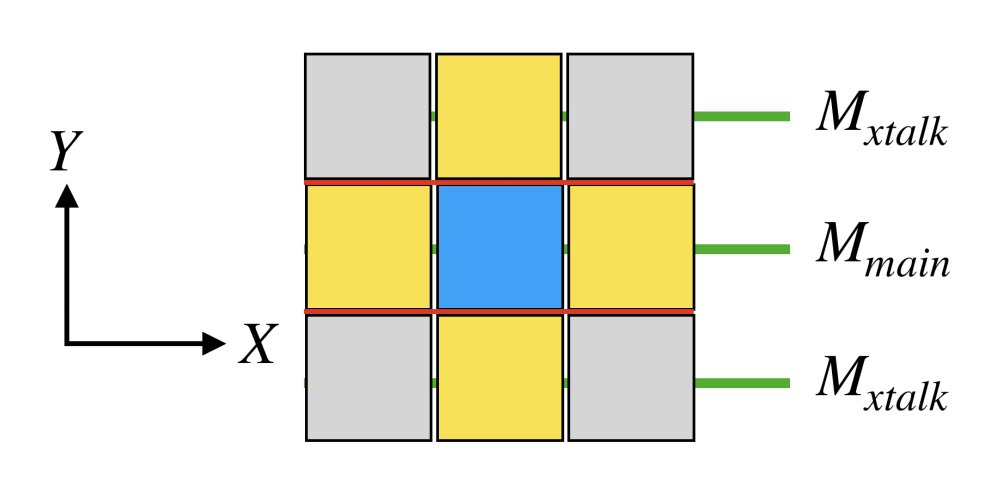
\includegraphics[width=\linewidth]{scnd_xt} \\ (a)
	\end{minipage}
	\begin{minipage}{0.33\linewidth}
		\centering
		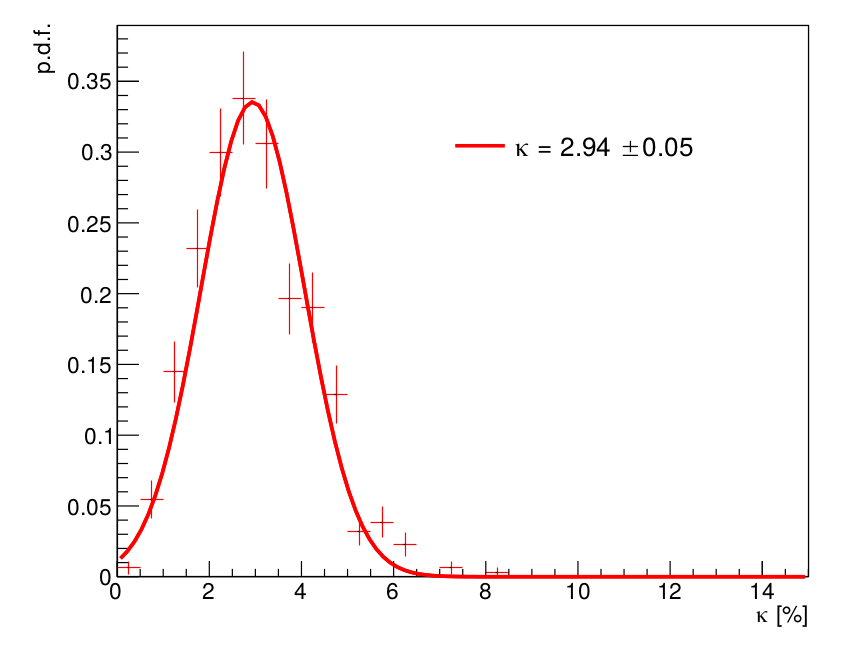
\includegraphics[width=\linewidth]{scnd_xt2} \\ (b)
	\end{minipage}
	\begin{minipage}{0.33\linewidth}
		\centering
		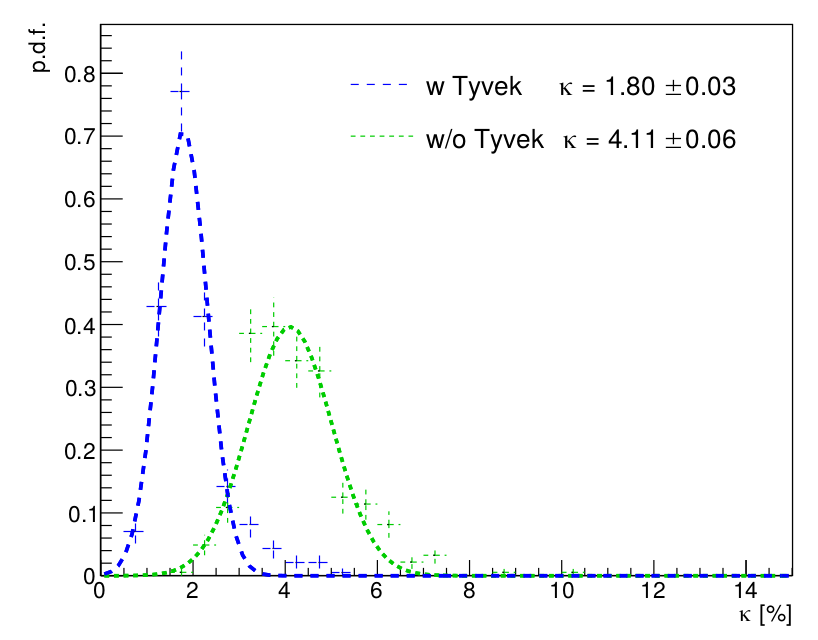
\includegraphics[width=\linewidth]{scnd_xt3} \\ (c)
	\end{minipage}
	\caption{The cross--talk scheme (a) and the measured probability (\autoref{eq:xt}) of the light migration to the neighbor cube (b) divided into the vertical and horizontal direction(c). The migration in vertical direction is suppressed with the Tyvek sheets.}
	\label{fig:sfgd:up:xt}
\end{figure}

\section{Conclusion}
The new scintillator target is going to be built for the upgrade of the near detector. It will be placed between two HA--TPCs. The detector is highly granular. The readout is organized from 3 surfaces making possible the 3D reconstruction of the events.

The performed beamtests demonstrate good detector performance for the processes of interest. High light yield and small time resolution were observed with the beam of charged particles with momentum O(1 GeV/c).

The setup opens a road towards sophisticated measurements of the neutrino interactions. First of all, the total fiducial mass in ND280 will be doubled providing many more statistics for the analysis. A high granularity allows the detection of the short nucleon tracks. Lower threshold for proton detection will allow us to reconstruct nearly all the protons produced in the neutrino interactions in ND280. With such a measurement, the resolution of the neutrino energy measurements will be improved. The new detector can distinguish a type of self-contained particle, thus it can measure neutrino interactions producing low momentum lepton and/or pion. In the current detector, TPCs are obligatory for particle type definition. A small time uncertainty and usage of the time-of-flight detectors provide a robust separation between particles going inside and outside the target. High granularity is useful for the separation between gamma conversion and electron production in neutrino interactions. Constrain the electron neutrino cross-section with the near detector can improve the precision of the oscillation analysis. Conversion of the gamma rays produced in neutrino interaction outside of fiducial volume is the main background for the process of interest and it can be severely suppressed in the new target.

With the SuperFGD, new analysis techniques may be developed to use all the benefits of the setup for neutrino studies. An example of an improved method of anti-neutrino energy reconstruction is presented in the next chapter.

\chapter{Neutron tagging in SuperFGD}
\label{ch:up:neutron}
A new detector opens a possibility for a new method of physics measurements. In this chapter I will discuss a method for an improved anti-neutrino energy reconstruction in the CCQE interactions $\overline{\nu}_\mu+p\to\mu^++n$. With the large mass of the SuperFGD detector (2 tons), neutrons are likely to scatter over the nucleon, producing charged particles. If the detector has good enough time resolution, neutron energy can be measured precisely with the time of flight. The time difference between muon production and neutron rescattering will indicate its energy. Knowledge about the hadron kinematics will gain the precision of anti-neutrino energy reconstruction. With the disbalance in the transverse kinematics of the muon and hadron, we can probe the nuclear effects. Such an analysis was performed for neutrino but was impossible for anti-neutrino as neutron detection efficiency was small.

We tested the possibility of neutron detection in a SuperFGD-like setup with different options considering detector time resolution. A possibility to measure neutron energy with reasonable uncertainty was demonstrated. The improvement of the anti-neutrino energy reconstruction was obtained. Overall, the method allows an interesting reduction of the strong correlations between the flux and the interaction models that arise in the measure of the neutrino oscillation probability and $\delta_{CP}$ phase.

\section{Motivation}
As was overviewed in \autoref{ch:T2K:general} the accurate measurements of the neutrino energy are essential for the precise oscillation analysis. Future experiments (DUNE, Hyper--Kamiokande) are very sensitive to the neutrino energy spectrum with their measurements of the CP violating phase $\delta_{CP}$. At the moment, T2K uses charged current quasi--elastic (CCQE) interactions to reconstruct neutrino energy. With the measured lepton momentum and direction and assuming known incoming neutrino direction and fixed liberation energy, the neutrino energy calculation is straight-forward. But such a measurement can be biased.
The bias is implemented with the initial movement of the target nucleons (Fermi motion) and liberation energy smearing. Also, mesonless neutrino interactions with multiple nucleons (mostly 2) will have different kinematics comparing to CCQE. The other source of bias is unreconstructed meson or a meson that was absorbed in the nucleus medium. These secondary interactions and multi-nucleons reactions are studied very poorly and the predictions of different models varies a lot. Even usage of the same detector at near and far sites can not solve the problem. Oscillated flux is different from the initial one, thus the proper model of neutrino interactions is essential to estimate the number of events at the far detector based on the measurements in the near detector.

To avoid the effects mentioned above, one can select a sample that is free from nuclear effects. The usage of the so--called ``transverse kinematic variables'' was theoretically motivated~\cite{Lu2016} and successfully implemented in the experiment~\cite{Abe2018d}. The detailed description of the method is provided in \autoref{sec:intro:pt} of \autoref{ch:nu_phys}. The implementation is straight forward for the neutrino interactions, where we expect to detect a muon and a proton in the final state $\nu_\mu+n\to\mu^-+p$. But it can not be directly applied for the anti-neutrino, where the charge--less neutron is produced. The SuperFGD--like detector can make possible effective neutron detection and energy measurements. Thus the transversal variables become measurable for anti-neutrino interactions as well.

In the hydrocarbon scintillator we have neutrino interactions over Hydrogen and Carbon only. Moreover interactions over Hydrogen are free from nuclear effects and prompts neutrino energy precisely. The transverse momentum for the interactions over these two elements in the SuperFGD with T2K anti-neutrino flux is shown in \autoref{fig:up:n:pt}. The interactions over Hydrogen are clearly separated from the Carbon ones. If we manage to measure $\delta p_T$ we will be able to extract a Hydrogen sample that is free from the nuclear effects and measure anti-neutrino energy precisely.

\begin{figure}[!ht]
	\centering
	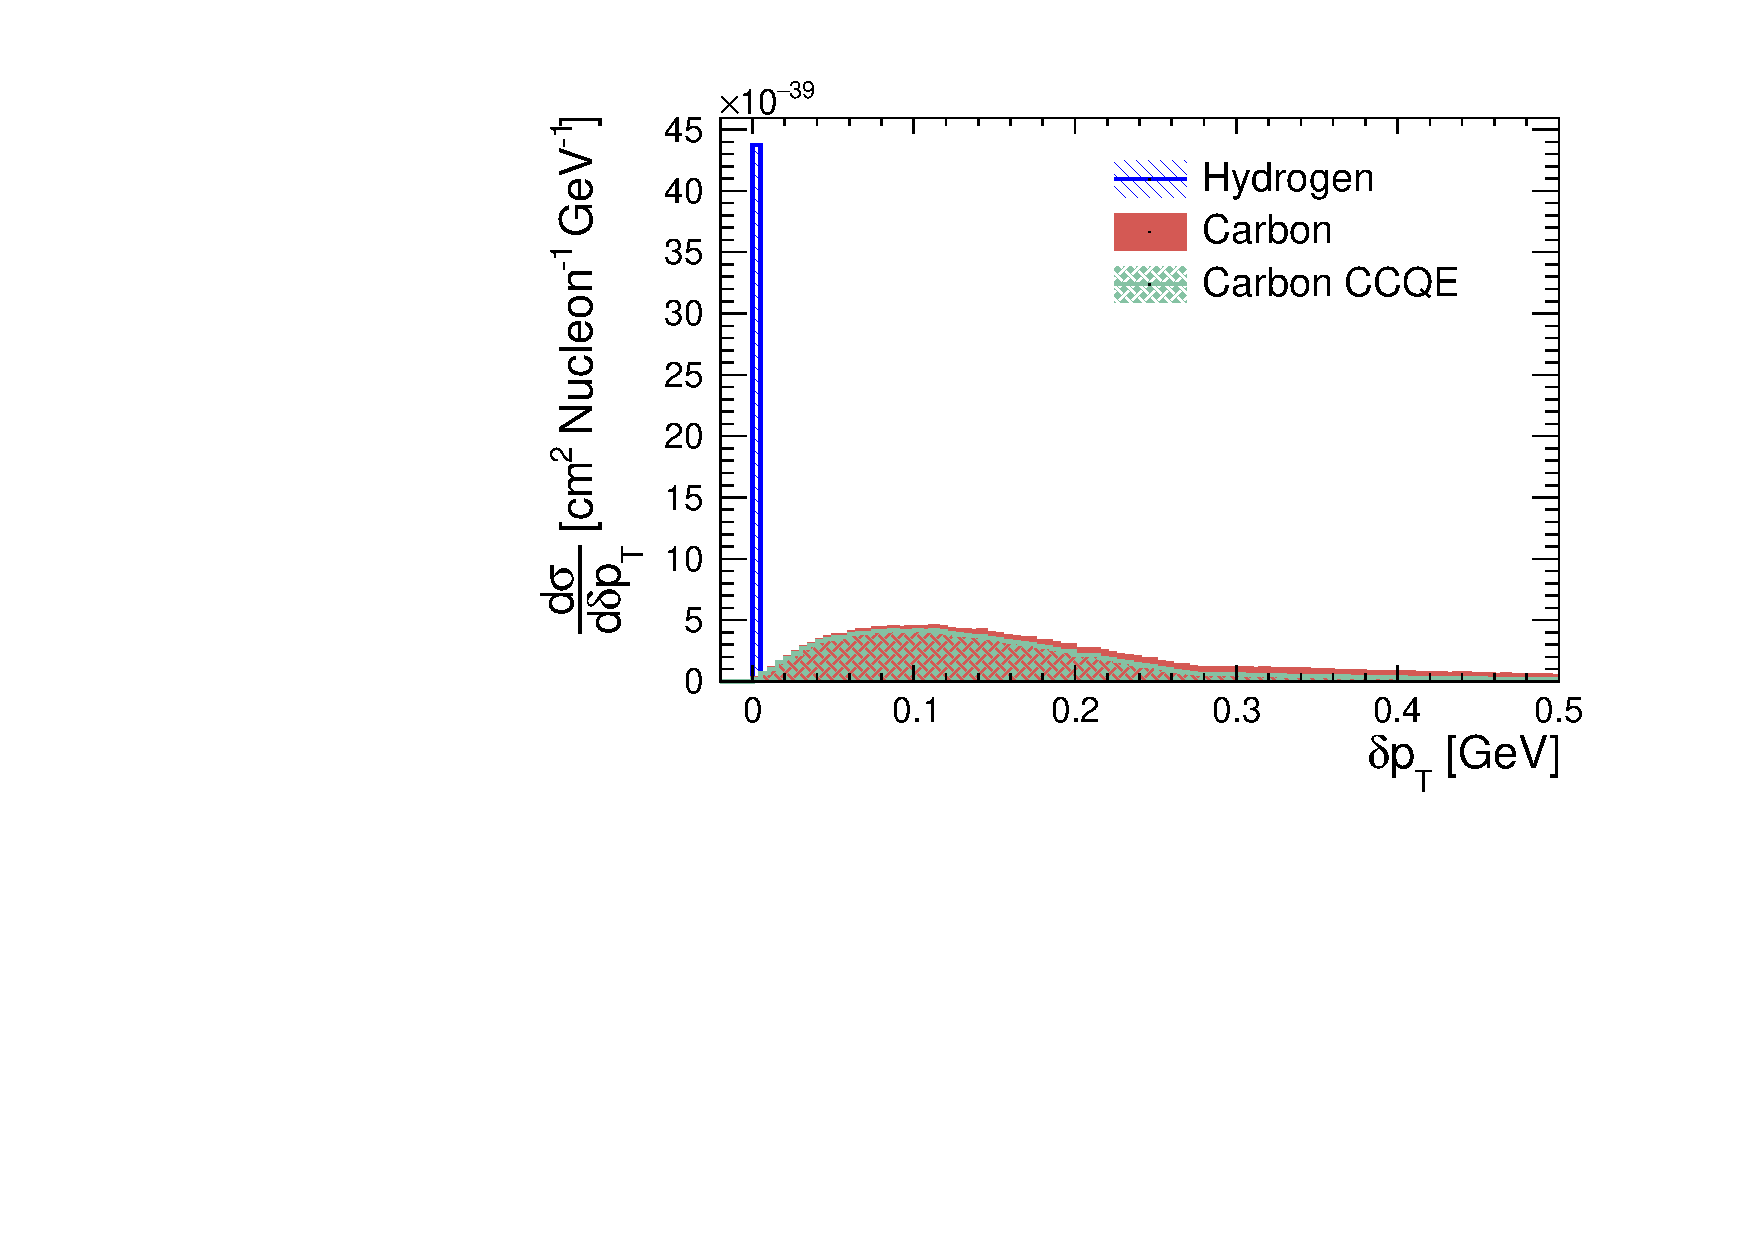
\includegraphics[width=0.6\linewidth]{pt}
	\caption{The differential cross section for $CC0\pi$ interactions on a hydrocarbon target as a function of $\delta p_T$ for anti-neutrino interactions from the T2K experiment’s anti-neutrino flux simulated with the NEUT generator. The samples are divided into the target nucleon and reaction type (for Carbon only).}
	\label{fig:up:n:pt}
\end{figure}

To measure the transversal momentum we need to estimate the neutron energy precisely. We are going to do it with the time of flight. The time of the neutron production can be measured accurately with the timing of a muon track. In the massive detector, a neutron is likely to scatter over the nuclei producing charged particles. The most common daughters are low energy protons and alpha-particles. Thus we expect a large light deposition from the stopping hadron that will allow accurate time measurement of the neutron scattering. With the end and start time references neutron velocity and thus energy can be easily reconstructed. The scheme of the process of interest is shown in \autoref{fig:up:n:top}.

\begin{figure}[!ht]
	\centering
	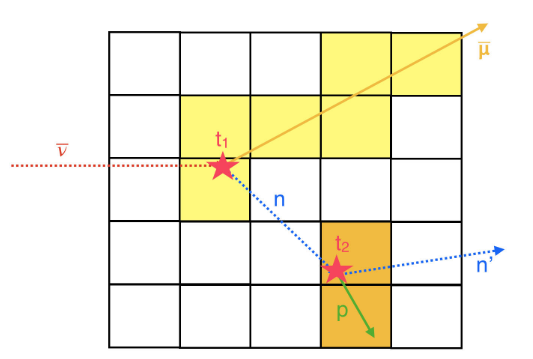
\includegraphics[width=0.5\linewidth]{n_top}
	\caption{The process of interest that is going to be used for the measurement of the neutron energy produced in neutrino interaction with the time of flight.}
	\label{fig:up:n:top}
\end{figure}

\section{Geant4 simulation}
We developed a simulation toolkit to study secondary interactions of the neutron produced in the anti-neutrino interactions. The simulation procedures discussed in \autoref{sec:up:sfgd_sim} of \autoref{ch:up:sfgd} are used. For the simplicity, we started with the particle gun samples with the neutron energy distributed uniformly from 0 up to 800 MeV. The starting position in the geometrical center of the detector is set. The neutron direction is distributed uniformly in $4\pi$ angle. Neutron interactions as well as interactions of secondary particles are carried by the Geant4 toolkit with ``QGSP BERT HP'' physics list that is widely used in HEP (e.g. ATLAS experiment). It uses quark gluon string model for the high energy events ($\geqslant$ 20 GeV) and Bertini cascade model for lower energies ($\leqslant$ 10 GeV). All the standard EM processes and decays are included. It also uses precise simulations of the low energy neutrons (E<20 MeV) cross-sections. The full chain of readout simulation including ionization energy loss by charged particles, Birks saturation, light attenuation in the fibers, MPPC efficiency is applied.

\subsection{Efficiency and energy resolution}
The first analysis output is a fraction of neutrons that produced particles that are further detected. The obtained efficiency is presented in \autoref{fig:up:n:eff}. The angular dependence comes from the detector asymmetry. X and Z dimensions are similar with \sfgdx{} and \sfgdz{} cubes but Y dimension is much smaller with \sfgdy{} cubes, thus less neutrons interact along this direction.

\begin{figure}[!ht]
	\centering
	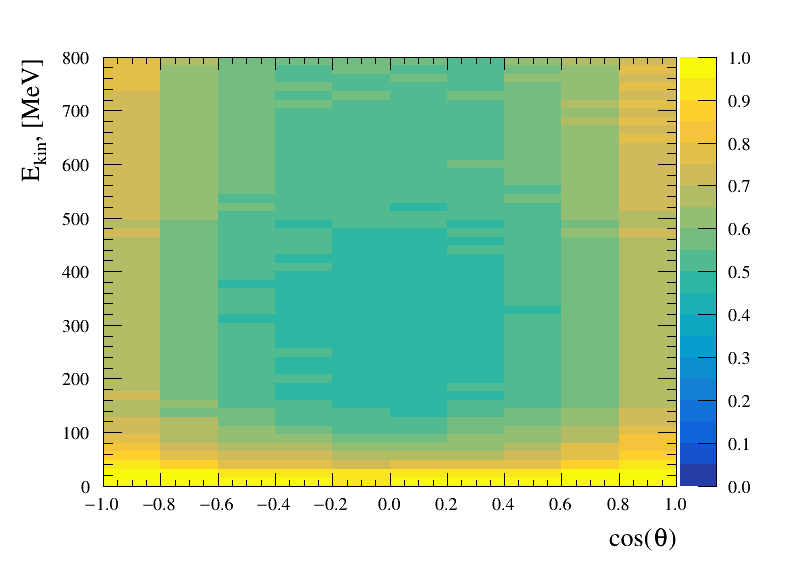
\includegraphics[width=0.6\linewidth]{eff}
	\caption{The efficiency of the neutron detection in the SuperFGD detector. Neutron particle gun was fired from the detector center isotropically. The angular dependence comes from the detector asymmetry.}
	\label{fig:up:n:eff}
\end{figure}

Neutron energy is measured with a time of flight method. Velocity is estimated based on the distance between two clusters in \autoref{fig:up:n:top} and measured time difference. Detector time resolution is expected to be the main source of the reconstructed energy smearing. The accuracy of the time measurements at the neutrino interaction vertex is assumed to be negligible as we will have large light deposition from the vertex activity and a long outgoing muon track that will provide lots of time measurements with illuminating many channels. Thus the time smearing in the neutron cluster is assumed to be the dominating uncertainty on the neutron energy reconstruction. In our study, we assume several options on the detector time resolution. Both estimations are based on the fact that the observed time resolution per MIP is 0.95 ns per channel. Then we apply corrections to estimate the precision of the time measurements of the stopping hadrons. The first method is based on the measured light yield from the neutron cluster. With higher light yield, a waveform grows faster and a deviation of the time delay between a signal and its registration is smaller. The measurements with precise digitizer observed a square root dependence of the time resolution on the light yield~\cite{Niemann2010}. As we measured 0.95 ns uncertainty per muon track that gives 40 p.e., we could extrapolate the uncertainty with the known dependence.

\begin{equation}
\label{eq:up:n:ly}
	\sigma^{ly}_t=0.95\text{ ns}/\sqrt{3}\cdot\sqrt{40 \text{ PE/LY}}, \hspace{2cm} \sigma^{ly}_t>200\text{ ps}
\end{equation}

The division by $\sqrt{3}$ shows the improvements in the measurement with 3 channels over the one channel. The bottom limit of 200 ps is set as further improvements are limited by the smearing in scintillator and fibers. Light emission by scintillator and light rescattering in fibers are not instant and provide some uncertainty.

This method is quite optimistic but the prototypes were not tested with the detection of large light emission. Thus to prevent an exaggeration of the energy resolution we considered a conservative estimation. If the measurements for each channel are independent their uncertainties can be sum up in quadrature. Thus the average uncertainty of N measurements will be $\sqrt{N}$ times more accurate than the single one.

\begin{equation}
\label{eq:up:n:ch}
	\sigma^{ch}_t=0.95\text{ ns}/\sqrt{\text{\#channels}}, \hspace{2cm} \sigma^{ch}_t>200\text{ ps}
\end{equation}

With the known model of the time resolution, I estimated the smearing of the reconstructed neutron energy. The results are presented in \autoref{fig:up:n:smear} a.

\begin{figure}[!ht]
	\centering
	\begin{minipage}{0.49\linewidth}
		\centering
		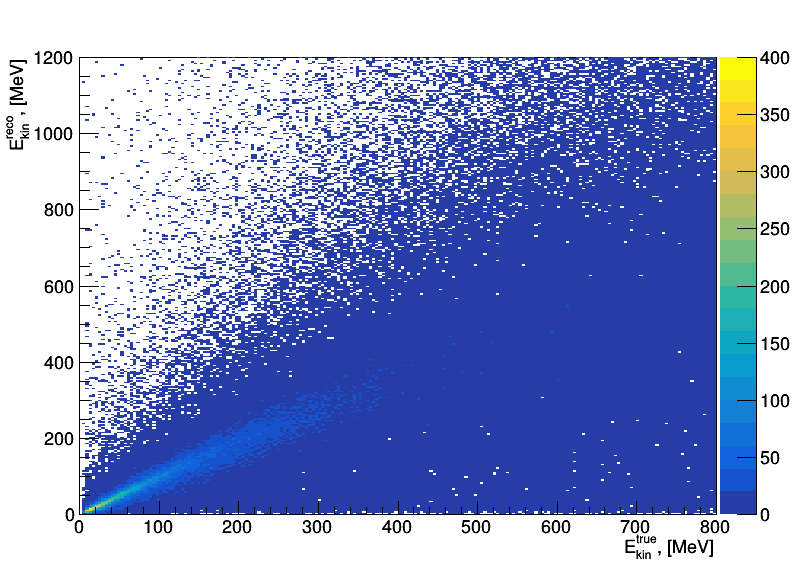
\includegraphics[width=\linewidth]{smear_0} \\ (a)
	\end{minipage}
	\begin{minipage}{0.49\linewidth}
		\centering
		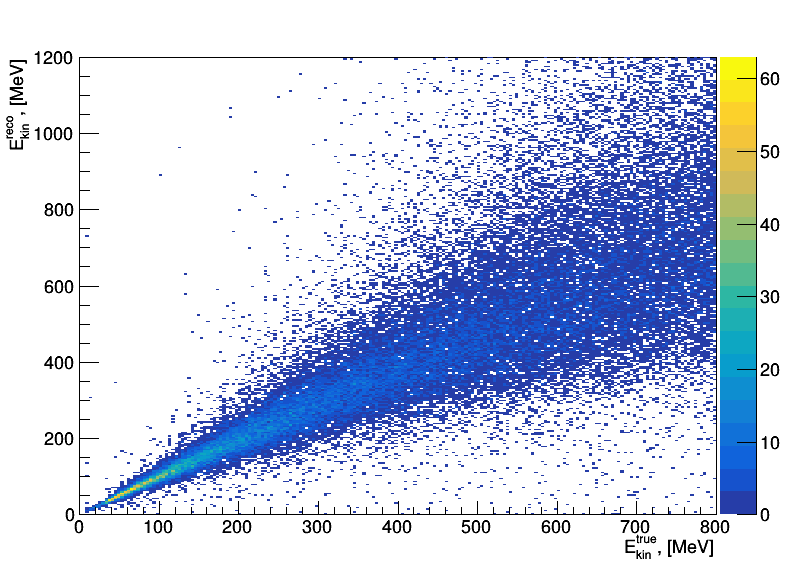
\includegraphics[width=\linewidth]{smear_50} \\ (b)
	\end{minipage}
	\caption{The neutron energy smearing for all neutrons (a) and for neutrons with travel distance more then 50 cm (b). The time resolution is estimated with \autoref{eq:up:n:ly}.}
	\label{fig:up:n:smear}
\end{figure}

The observed smearing is quite severe. There are two main sources of such a large resolution. The first one is neutrons with a short travel distance. The time resolution is similar for all neutron interactions, but at a small distance it affects energy estimations more significant. A cut on the travel distance can gain the resolution. The distribution of the neutron travel distance with respect to its energy is shown in \autoref{fig:up:n:e_dist}. I am also accepting all the neutron clusters disregard the light yield. Events with a very low level of signal provide an enormous large smearing and should be also excluded. The time resolution estimated based on the light yield is shown in \autoref{fig:up:n:time} b. The discrete peaks come from the events with a small number of photoelectrons (1 p.e - 3.29 ns, 2 p.e - 2.45 ns, etc.)

\begin{figure}[!ht]
	\centering
	\begin{minipage}{0.4\linewidth}
		\centering
		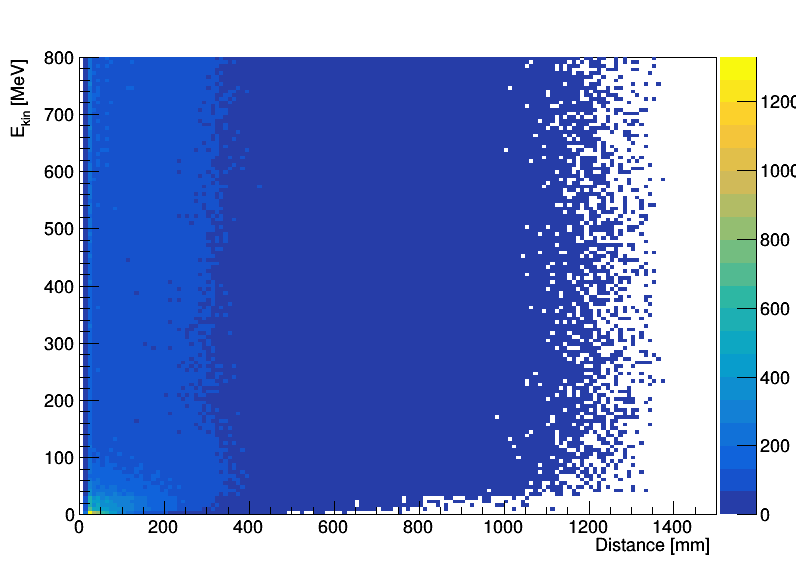
\includegraphics[width=\linewidth]{e_dist}
    \caption{The neutron travel distance until the scattering with respect to its initial energy.}
    \label{fig:up:n:e_dist}
	\end{minipage}
	\begin{minipage}{0.19\linewidth}
	\hspace{\linewidth}
	\end{minipage}
	\begin{minipage}{0.4\linewidth}
		\centering
		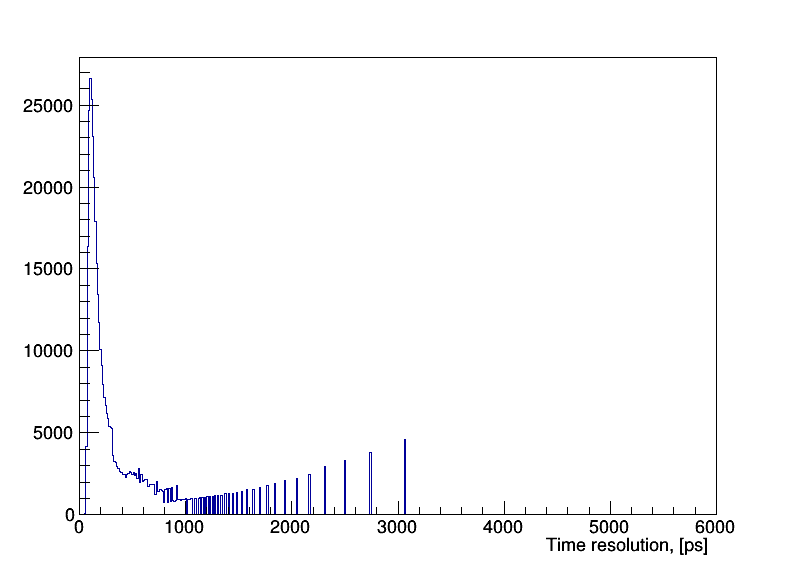
\includegraphics[width=\linewidth]{time_n}
    \caption{The estimations on the time resolution for the neutron clusters.}
    \label{fig:up:n:time}
	\end{minipage}
\end{figure}

The cut on the light yield at the level of 40 p.e. was set to provide a time resolution not worth than for a MIP particle. I also studied the dependence of the energy resolution and detection efficiency with different lever arm cuts. The effect of the resolution improvement with the larger travel distance cut is shown in \autoref{fig:up:n:res}. The efficiencies for 20 cm and 70 cm lever arm cuts are shown in \autoref{fig:up:n:eff2}.

\begin{figure}[!ht]
	\centering
	\begin{minipage}{0.49\linewidth}
		\centering
		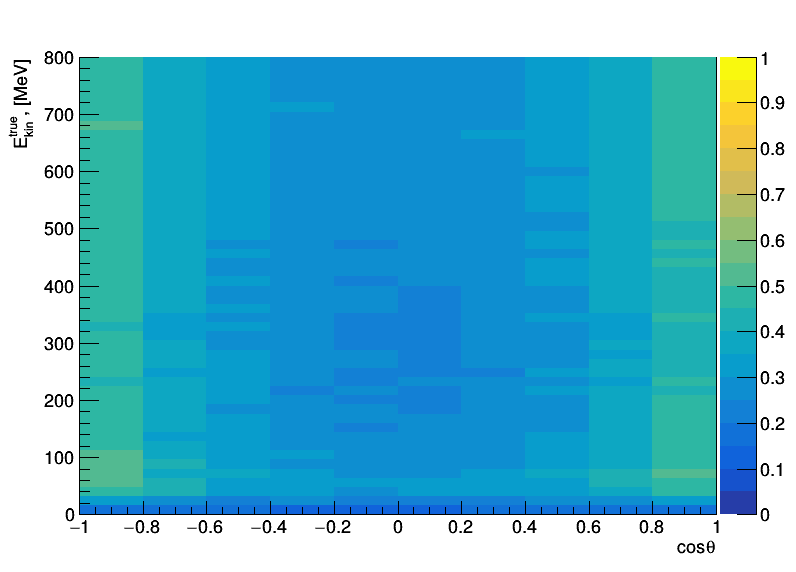
\includegraphics[width=\linewidth]{eff_20} \\ (a)
	\end{minipage}
	\begin{minipage}{0.49\linewidth}
		\centering
		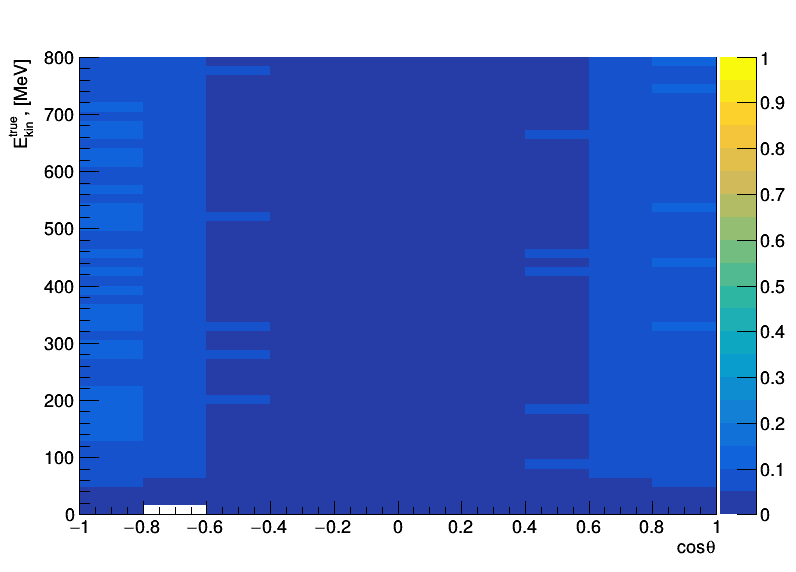
\includegraphics[width=\linewidth]{eff_70} \\ (b)
	\end{minipage}
	\caption{The efficiency of the neutron detection with the cut on the travel distance at 20 cm (a) and 70 cm (b).}
	\label{fig:up:n:eff2}
\end{figure}

\begin{figure}[!ht]
	\centering
	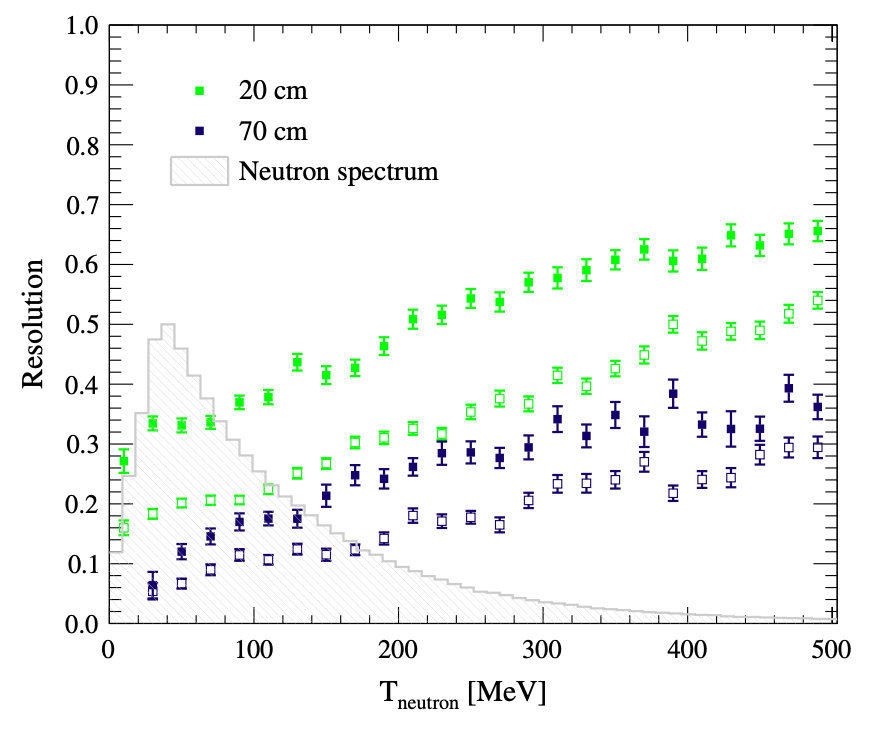
\includegraphics[width=0.5\linewidth]{res_spec}
	\caption{The neutron kinetic energy resolution as a function of the its kinetic energy, assuming different lever-arm cuts (20 cm and 70, denoted by differing colors) and timing resolutions. The hollow markers correspond to a timing resolution using \autoref{eq:up:n:ly}, while the filled markers correspond to \autoref{eq:up:n:ch}. The resolution is taken as the ratio of the largest of the two standard deviations to the mean of a double-sided Gaussian fitted to the reconstructed neutron kinetic energy in a bin of true neutron kinematic energy. The gray band shows NEUT 5.4.0’s predicted distribution of neutron kinematic energies for CC0π neutrino interactions using the T2K experiment’s anti-neutrino flux.}
	\label{fig:up:n:res}
\end{figure}

\section{Background estimations}
In the method described above, we assumed the isolated cluster was originated by the neutron from the neutrino interaction. This analysis may be affected by the out of fiducial volume backgrounds when a photon or neutron produced outside SuperFGD interacts inside the detector. Such a cluster can not be separated from the interaction of the neutron produced by the anti-neutrino interaction inside SuperFGD. I estimated the rate of such a pileup and compared the signal and the background. A similar technique to what was used in \autoref{sec:up:sfgd:pu} is used to generate the OOFV sample. I studied the time delay between the anti-neutrino interaction in SuperFGD and the neutron cluster detection versus the lever arm for both signal and background samples. The resulting distribution is presented in \autoref{fig:up:n:bg}. One can see the large difference in the distributions of both samples. The rate of background events is small.

\begin{figure}[!ht]
  \centering
  \begin{minipage}{0.49\linewidth}
    \centering
    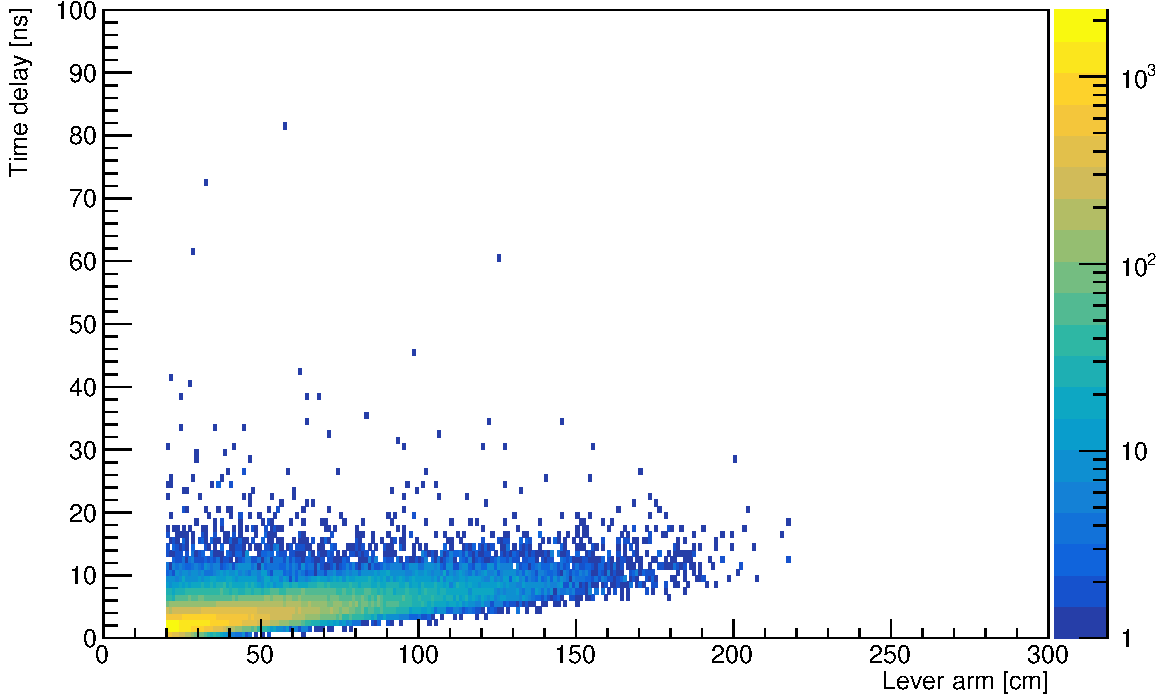
\includegraphics[width=\linewidth]{signal_LA_T} \\ (a)
  \end{minipage}
  \begin{minipage}{0.49\linewidth}
    \centering
    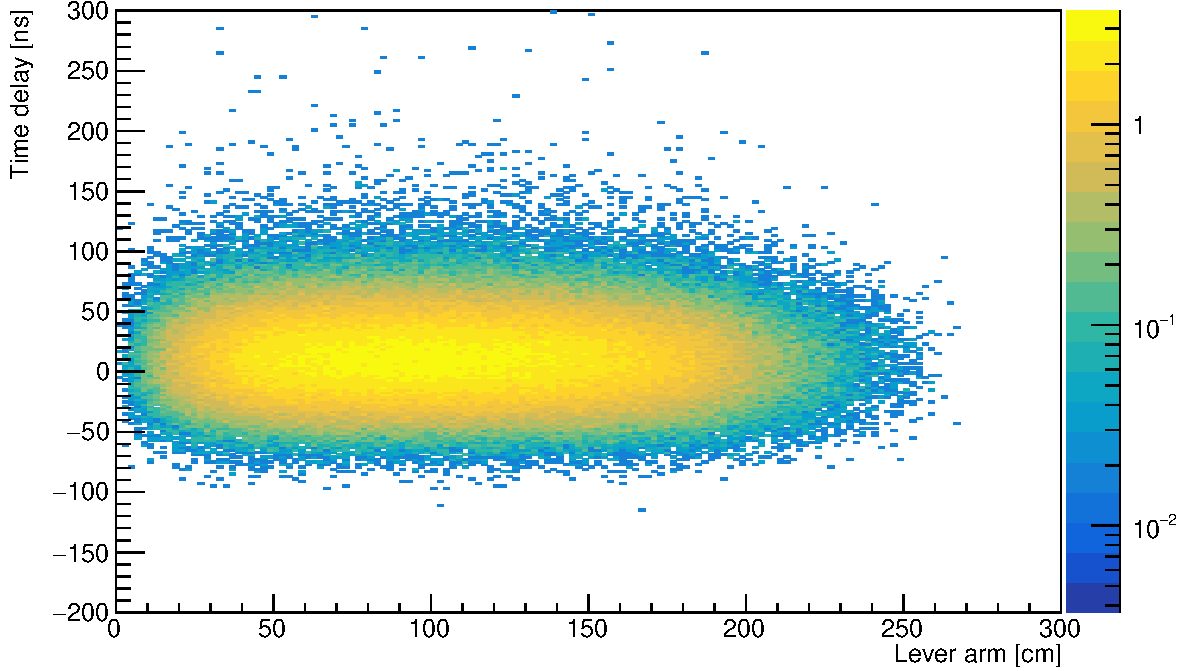
\includegraphics[width=\linewidth]{BG_LA_T} \\ (b)
  \end{minipage}
  \caption{The distribution of the time delay between the anti-neutrino interaction in SuperFGD and neutron cluster detection versus the distance between them for the signal events (a) and out of fiducial volume interactions (b) normalized to the number of signal events.}
  \label{fig:up:n:bg}
\end{figure}

I merged these samples event by event to study the purity of the neutron detection. The time structure of the neutrino interactions was taken the same for both samples. We assumed the bunches are Gaussian with $\sigma=19$ ns.  The first isolated cluster that was found after the anti-neutrino interactions is considered as a neutron detection. If it is caused by the OOFV interaction it will be marked as a background otherwise it is a signal. Based on this classification the purity was estimated. I found that with such a method it is very unlikely to misinterpret the background as a signal. The main reason is the overall low background rate. The other one is usually large difference in time between neutrino interaction and a cluster from a background neutron. A signal neutron interacts faster in time. The obtained purity is presented in \autoref{fig:up:n:pur}.

\begin{figure}[!ht]
  \centering
  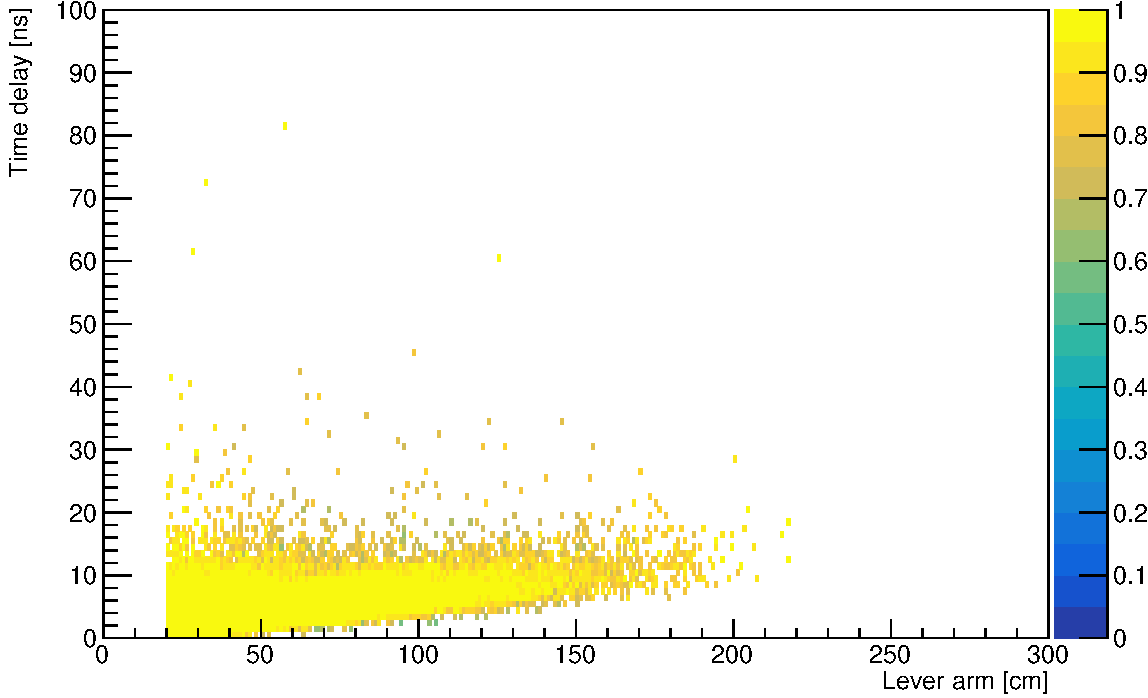
\includegraphics[width=0.5\linewidth]{purity}
  \caption{The purity of the neutron cluster selection. The contamination of the neutral particles produced OOFV is proved to be small.}
  \label{fig:up:n:pur}
\end{figure}


\section{Prospects for physics}
The main goal of the current study is a more sophisticated measurement of neutrino interactions. We performed a simulation to evaluate how neutron detection may gain accuracy. The sample of the CC0$\pi$ events was generated using NEUT 5.4.0. Only events with muon momentum higher than 100 MeV/c are considered as it is an expected threshold of the muon detection in the SuperFGD. Lepton detection is essential for the proper identification of neutrino type and flavor. Plenty of smearings was applied to the simulation to estimate the detector output. Muon momentum was smeared by 4\% with a Gaussian distribution. The value comes from the typical resolution of the TPC in the ND280. The angle of the outgoing muon is smeared with 1${}^\circ$ driven by the granularity of the scintillator detector. The neutron kinematics is smeared according to the results of the GEANT4 simulations described in the previous sections.

After incorporation of all the smearing effects, we can estimate the output of the measurements with SuperFGD. The distribution of the transversal momentum $\delta p_T$ is shown in \autoref{fig:up:n:dpt_sim}. Comparing this figure to \autoref{fig:up:n:pt} we can see the effect of the detector smearing. However, the hydrogen sample is largely distinct from the Carbon one.

\begin{figure}[!ht]
  \centering
  \includegraphics[width=0.5\linewidth]{pt_sim}
  \caption{The NEUT 5.4.0 predicted event rate of CC0$\pi$ interactions from the T2K anti-neutrino flux as a function of $\delta p_T$ obtained after applying the detector smearing effects. The detector time resolution is estimated with \autoref{eq:up:n:ly}.}
  \label{fig:up:n:dpt_sim}
\end{figure}

In our analysis, we are trying to find the best value of the cuts on lever arm and $\delta p_T$ to maximize the improvement of neutrino energy reconstruction precision. All the events with $\delta p_T$ below the cut value are supposed to be the interactions over Hydrogen. The efficiency and purity of such a selection for different lever arms and cut values are shown in \autoref{fig:up:n:opt}. For this particular figure the detector resolution was estimated with \autoref{eq:up:n:ly}. If I use \autoref{eq:up:n:ch} instead, the shape will be the same but the purity will be approximately 10\% smaller. A good compromise was found with cuts $\delta p_T < 40$ MeV/c and $L < 10$ cm. The resulting Hydrogen purity and efficiency are 61\% and 22\% respectively. With the full T2K-II statistics we expect around 26 thousand interactions in SuperFGD.

\begin{figure}[!ht]
  \centering
  \includegraphics[width=0.5\linewidth]{eff_pur}
  \caption{The anti-neutrino hydrogen purity vs efficiency for different $\delta p_T$ and lever-arm cuts. The first (top left) marker on each line corresponds to a 10 MeV cut and then the star corresponds to the chosen $\delta p_T$ cut of 40 MeV. Each line corresponds to a different lever-arm cut and is made using \autoref{eq:up:n:ly} to determine the time resolution.}
  \label{fig:up:n:opt}
\end{figure}

From \autoref{fig:up:n:opt} one can see that a stronger lever arm cut sharply reduces the efficiency, but not improving the purity. This happens because of the correlation between the neutron energy and travel distance. Most of the neutrons produced in ND280 in anti-neutrino interactions are below 100 MeV (\autoref{fig:up:n:res}). In this region the travel distance increase with the growing energy (\autoref{fig:up:n:e_dist}). Therefore, a longer lever arm cut accepts more energetic thus faster neutrons and the energy resolution is not improving. The best performance is expected with the lever arm cut set to 10 cm and $\delta p_T$ cut set to 50 MeV. The events passing the cuts are further used to reconstruct anti-neutrino energy under the assumption of CCQE interaction.

\begin{equation}
  \label{eq:n:energy}
  E_\nu=\frac{m^2_n-m^2_p-m^2_\mu+2m_p E_\mu}{2\left(m_p-E_\nu+p_\mu \cos\theta_\mu\right)}
\end{equation}

The smearing of the reconstructed energy with and without $\delta p_T$ cut is shown in \autoref{fig:up:n:smear_nu}. It was observed that the additional information from the neutron ToF improves the anti-neutrino energy reconstruction precision from 15\% to around 7\%.

\begin{figure}[!ht]
  \centering
  \begin{minipage}{0.49\linewidth}
    \centering
    \includegraphics[width=\linewidth]{eKinNoCut} \\ (a)
  \end{minipage}
  \begin{minipage}{0.49\linewidth}
    \centering
    \includegraphics[width=\linewidth]{eKinWCut} \\ (b)
  \end{minipage}
  \caption{The reconstructed energy of anti-neutrino under the CCQE assumption with \autoref{eq:n:energy} before applying lever arm and $\delta p_T$ cut (a) and after (b). The Z-axis is normalized such that the highest value in each plot is one.}
  \label{fig:up:n:smear_nu}
\end{figure}

The key feature of the transversal variables is the measurements that are independent of the poorly understood nuclear effects. To prove that the selected sample depends weakly on the theoretical models we estimated anti-neutrino energy resolution with various 2p2h normalization and with different models of the initial nucleon momentum. The results of these cross-check is shown in \autoref{fig:up:n:model}. One can see that solid lines that are obtained after the applying of cuts demonstrate much weaker dependence on the input parameters. Relatively large changes in the normalization of the interactions with two particles don't degrade the neutrino energy resolution at all. Thus the proposed method provides precise measurement of the neutrino energy and is poorly affected by nuclear effects.

\begin{figure}[!ht]
  \centering
  \begin{minipage}{0.49\linewidth}
    \centering
    \includegraphics[width=\linewidth]{2p2h_sim} \\ (a)
  \end{minipage}
  \begin{minipage}{0.49\linewidth}
    \centering
    \includegraphics[width=\linewidth]{model_sim} \\ (b)
  \end{minipage}
  \caption{Accuracy of the reconstructed anti-neutrino energy after applying the lever arm and $\delta p_T$ cuts. The dependence on the 2p2h normalization (a) and initial nucleon momentum model (b) is shown. The solid lines corresponds to the measurement after the cuts $L>10$ cm $\delta p_T < 50$ MeV/c, the dashed lines are obtained before the cuts.}
  \label{fig:up:n:model}
\end{figure}

\section{Conclusion}
The proposed method demonstrates the ability of the new scintillator detector SuperFGD to measure neutrons produced in the anti-neutrino interactions. neutron energy can be measured with a relatively small uncertainty with the time of flight method. This information can be further used to compute the transversal kinematic imbalance of the neutrino interaction. The sample that is nearly free from nuclear effects can be selected with the requirement of low $\delta p_T$ value. This method has a strong advantage as it is sensitive to both the shape and normalization of the neutrino energy spectrum. Other flux--constraining methods are mainly sensitive to the normalization only. The constraints on the flux shape for both neutrino and anti--neutrino are essential for precise measurements of the $\delta_{CP}$ phase.

In this particular study, proton kinematics is not used. We do not expect a proton to be produced in the CCQE interaction but it can be born due to nuclear effects. The measurements of the stopping hadrons can be performed precisely with a highly granular SuperFGD detector. Thus the further precision improvement is possible with additional information.

We concentrated on the CC0$\pi$ topology in the analysis, while CC1$\pi$ topology can be also very promising. The $\delta p_T$ in this case will be calculated taking into account all the particles in the final state. In particular, CC1$\pi^0$ interactions can be used with detection of the isolated $\pi^0$ in the final state $\overline{\nu}_\mu+p\to\mu^++n+\pi^0$. In case when we have three particles in the final state a deeper analysis can be performed with double transversal kinematic parameters $\delta p_{TT}$ (\autoref{sec:intro:pt} of \autoref{ch:nu_phys}).

The performed analysis was published in~\cite{Munteanu2019}.

\end{document}